\documentclass[twoside,a4paper,11pt]{article}

\usepackage{amssymb}%Blacksquare
\usepackage[margin=2cm]{geometry}
\usepackage{amsmath,amssymb}
\usepackage{parskip,graphicx} 
\usepackage[makeroom]{cancel} %used to cross out terms in equations
\usepackage[utf8]{inputenc} %not clear effect
\usepackage[T1]{fontenc} %not clear effect
\usepackage[english]{babel}% not clear effect
\usepackage{float} %used for fixed tables with [H]
\floatstyle{plaintop} %used to place table caption on top
\restylefloat{table}

\usepackage[document]{ragged2e} %used to justify text
\usepackage{amsthm}
\usepackage{commath}
\usepackage{textcomp}
\usepackage{enumerate}
\usepackage{wrapfig}
\usepackage{epstopdf}
\usepackage{subfig}
\usepackage[font=small,labelfont=bf,
   justification=justified,
   format=plain]{caption}
\usepackage{array}% http://ctan.org/pkg/array	
\usepackage{breqn} %used to split equations on multiple lines
\usepackage{listings}
\usepackage{pdfpages} %used to include pdfs

\usepackage{eufrak} %used for fancy math font

\usepackage{multicol} %used for multicolomns

\usepackage{dsfont} %for unity element 

\usepackage{siunitx} %used for units

\usepackage{titlesec}
\usepackage[titletoc,toc,title]{appendix} %used for apendix

\newcommand\numberthis{\addtocounter{equation}{1}\tag{\theequation}} %used for numbering only one equation 

\usepackage{braket} %quantum brackets
\DeclareMathAlphabet\mathbfcal{OMS}{cmsy}{b}{n}%caligraphy font

\numberwithin{equation}{section}

%used for pointing at equations
\usepackage{pst-node}
\usepackage{tikz-cd} 

\usepackage{tikz}
\usetikzlibrary{tikzmark}




\usepackage[nottoc]{tocbibind}

\usepackage{comment}
\usepackage{fancyhdr}

\newcommand{\parl}{\overset{\leftarrow}{\partial}}
\newcommand{\parr}{\overset{\rightarrow}{\partial}}

%used for boxing equations
\usepackage{empheq}
\usepackage{xcolor}
\definecolor{lightgreen}{HTML}{90EE90}
\newcommand{\boxedeq}[2]{\begin{empheq}[box={\fboxsep=6pt\fbox}]{align}\label{#1}#2\end{empheq}}

%used for disjoint unions
\newcommand{\cupdot}{\mathbin{\mathaccent\cdot\cup}}

\usepackage{tcolorbox}
\tcbuselibrary{theorems}

\newtcbtheorem{futwork}{Future work}%
{colback=white,colframe=white,coltitle=black,fonttitle=\bfseries}{fw}


\usepackage[hidelinks]{hyperref} %Used to hyper reference.Usually it has to be the last package to be imported, but there might be some exceptions to this rule.

\pagestyle{fancy}
\fancyhf{}
\fancyhead[R]{\rightmark}
\fancyhead[L]{Canonical Quantization and Time-Energy Uncertainty}
\fancyhead[LE,RO]{\thepage}
\renewcommand{\headrulewidth}{0.4pt}



\begin{document}
\pagenumbering{roman}



\begin{titlepage}
 
\begin{center}
 
\begin{figure}[H]
\centering
\includegraphics[width=0.4\linewidth]{Pics/jacobslogo.jpg}
\end{figure}
\vspace{10mm}
\LARGE
\text{Jacobs University Bremen} \\
\text{Department of Physics and Earth Sciences}
 
\vspace{25mm}
\textbf{\huge{Canonical Quantization Procedure and Time-Energy Uncertainty}} \\
 
\vspace{30mm}
\Large{BSc Thesis in Physics}\\
\vspace{10mm}
\large{as part of the courses}\\
\vspace{5mm}
\large{CA08-200303 Project Physics \\ CA08-200304 Thesis Physics}\\
\vspace{7.5mm}

by \\
\vspace{7.5mm}

\Large{\textbf{Daniel Prelipcean}}
\end{center}

\vfill

\large{Bremen, \today\\
\textit{Supervisor:} Prof. Dr. Peter Schupp\\
\textit{2$^{nd}$ Reader:} Prof. Dr. S{\"o}ren Petrat}


\vspace{2cm}

\end{titlepage}


 \newpage
	
\vspace*{\fill}
\begin{center}
\textbf{\large Abstract:}
\justify
A fresh interpretation of the Canonical Quantization Procedure of the Relativistic Bosonic Point Particle is presented by promoting coordinate time $t = x^0$ to an operator and introducing a new scalar parameter $\lambda$. The system time evolution is given via the linear  Schr{\"o}dinger equation in parameter time, $\hat{H} \ket{\psi} = \partial_\lambda \ket{\psi}$. The novelty consists in viewing the physical wave functions as being parameter-time independent solutions with mass eigenvalues, which can be used to construct off mass-shell states. Employing Ordinary Quantum Mechanics in a relativistic setting, this treatment can be viewed as a toy model of Quantum Gravity, and thus, faces similar issues that can be fortunately resolved, such as non-trivial time evolution and probability interpretation. In particular, it offers an axiomatic derivation of the time energy uncertainty relation.
\end{center}
\vspace*{\fill}
\iffalse


Quantization procedures, in particular for constrained systems like the point particle, were investigated in order to derive and interpret the Time Energy Uncertainty Relation (TEUR). Two reviews, one of canonical quantization procedures and one of the TEUR, are presented. The canonical quantization of the free relativistic point particle is carried out in a general background, as well as deformation quantization in a static background. Future work includes obtaining uncertainty relations in deformation quantization and its generalization for some explicit metrics, as well as to investigate other minor inconsistencies in the canonical approach.
\fi

\newpage

\setcounter{tocdepth}{3}
\tableofcontents

\newpage
\justify

\pagenumbering{arabic}
\setcounter{page}{1}


\section{Introduction}

Rigorous formalism often comes only after the discovery process, and not during or before. A mystery still standing is the derivation and interpretation of the Heisenberg time-energy uncertainty relation. Compared to the the position-momentum uncertainty relations, the time-energy one lacks a solid mathematical derivation, such as those given by Heisenberg \cite{HeisenbergUR}  or Robertson \cite{RobertsonUR}. It may still be possible that we understand a theory perfectly well physically, such that mathematical rigor is unnecessary. However, this is clearly not the case for Quantum Mechanics and its non-intuitive phenomena. Nevertheless, I strongly advocate for a clear mathematical structure justifying the variety of heuristic notions physicists use when describing physical phenomena.

Since the introduction of the uncertainty relation between position and momenta operators by Heisenberg \cite{HeisenbergUR}, a controversial issue has been the time-energy commutation relation that gives the time-energy uncertainty relation:
\begin{equation}
    Et - tE = -i\hbar \qquad \Rightarrow \qquad  \Delta E \Delta t \geq  \hbar/2
\end{equation}
This was not a mathematical derivation, but an intuitive assumption based on analogy, and it already introduced confusion as one noted by Busch \cite{BuschTEUR}, since  it suggests the existence of a time operator. Different types of time-energy uncertainty relations do indeed hold depending on the context, that is, interpretation of what time means (such as preparation time \cite{AharonovBohm}, characteristic time \cite{MandelstamTEUR}, lifetime, etc.). On the other hand, some Gedankenexperiments  disprove the time energy uncertainty, e.g. Einstein`s photon box in his debates with Bohr. Therefore, a unique universal time-energy uncertainty similar to the position-momentum does not exist and we shall formalize one in this thesis, as a major side-result.

By investigating Quantum Mechanics in a Relativistic setting, time is put on equal setting with space and becomes a canonical variable with the Hamiltonian as conjugated momentum, both promoted to operators. The canonical uncertainty relations then \cite{HeisenbergUR} hold axiomatically, and in particular:
\begin{equation}
   \Delta \hat{E}  \cdot \Delta \hat{t}  \geq \frac{\hbar }{2}
\end{equation}
However, a scalar parameter, usually taken to be proper time $\tau$, is needed to give the time evolution of the system. Since coordinate time $t$ is now an operator, we introduce a new parameter time $\lambda$ variable, that parametrizes the world line of a particle. Consequently, we are morally compelled to study the relationship between $\lambda$, proper time $\tau$ and coordinate time $t$.

Different approaches to combine Quantum Mechanics (QM) with General Relativity (GR) have been made (such as Loop Quantum Gravity or String Theory), but the "Holy Grail" of Theoretical Physics is yet to be found as any attempt of treating QM relativistically presents intrinsic inconsistencies. Moreover, a vast array of physically relevant results from either two theories do not hold in the joint picture. The first and most important issue is the Problem of Time, which occurs because \textit{time} takes a different meaning in each of QM and GR. It can be summarized as a vanishing Hamiltonian $H$ on wave functions, implying a static universe with no time evolution. A quite philosophical review of this issue is presented by Anderson \cite{AndersonTimeQG}, debating the meaning and the use of different time interpretations. 

The fresh perspective of this thesis is the reinterpretation of the above constraints (e.g. the physical mass-shell $H = p_\mu ^\mu + m^2$) as parameter time-independent equations, solved by physical wave functions. General wave functions can then be constructed as distributions thereof, resolving a great number of the issues aforementioned. In particular, the treatment presented in this paper reconciles  time interpretations in both Quantum Mechanics and (Special) Relativity, and implicitly yields a sound derivation of the time-energy uncertainty relation.

This thesis is organized as follows. Section \ref{sec:TimeQgrav} presents a short review of possible Quantization Procedures, and the Problem of Time that arises in combining Quantum Mechanics and General Relativity.  Section \ref{sec:relaprticleaction} shows how even the most simple case (a single particle in a gravitational background) implies a static universe. The new proposed approach of this thesis is presented in section \ref{sec:staticworldinterpretation}, where a novel interpretation of the mass-shell condition is given and its physical implications investigated. Further discussion, results and future outlook are given in section \ref{sec:discussion}.

\newpage
\section{The Problem of Time in Quantum Gravity}
\label{sec:TimeQgrav}

Quantization is the transition \textit{from} the classical analysis of physical phenomena to a newer understanding known as Quantum Mechanics. Considering that the world is truly quantum and the everyday world represents the "classical" limit, one finds that the quantization process is not unique, i.e. one needs to add several concepts and can do so along different paths.
The three logically sound paths to quantization developed so far are:
\begin{enumerate}
    \item  
The Canonical Quantization Procedure, which attempts also to preserve the formal structure of the classical theory, to the greatest extent possible. 

\item 
Path Integrals, conceived by Dirac and developed by Feynmann, involving a functional integral over all topologically allowed trajectories to compute a quantum amplitude.

\item
Deformation Quantization or Phase-Space Formulation, based on Wigner's quasi-distribution function and Weyl's correspondence between quantum-mechanical operators and ordinary phase-space functions.
\end{enumerate}

\begin{figure}[H]
    \centering
    
\[ \begin{tikzcd}
\mathcal{L} \arrow{r}{LT} & H \arrow{r}{Quant.} \arrow[swap]{d}{Red.} & \hat{H} \arrow{d}{Red.} \\%
& \tilde{H} \arrow{r}{Quant.}&  \tilde{\hat{H}}
\end{tikzcd}
\]
    \caption{The usual starting point is the Lagrangian $\mathcal{L}$, whence one derives the Hamiltonian $H$ via a Legendre Transformation (LT). Next, Quantization and Reduction to the physical phase-space (for constrained systems) have to be performed. The question, which now arises, is whether Quantization and Reduction commute or not. This is yet to be fully answered. Moreover, the Legendre transformation itself may impose problems.}
    \label{quantizationscheme}
\end{figure}
Further quantizations were also proposed (e.g. Enhanced Quantization, Klauder \cite{klauderquantization}), along with completely different interpretations of Quantum Mechanics (e.g. Cellular Automaton, 't Hooft \cite{hooftCA}).

\subsection{Canonical Quantization and Explicit Quantization Schemes}
The Canonical approach is inspired from the Hamiltonian approach to classical mechanics, in which a system's dynamics is generated via canonical Poisson brackets. The Canonical approach to Quantum Mechanics can be summarized by asserting that the classical Poisson brackets are promoted to commutators. Mathematically, this represents finding a quantization map $Q$ such that any function on the classical phase-space gets promoted to an operator $\hat{Q}_f$:
\begin{equation}
    \{Q_f,Q_g\} \rightarrow \frac{1}{i\hbar } [ \hat{Q}_f, \hat{Q}_g ]
\end{equation}
The following properties are desirable \cite{Qproperties} for the quantization map $Q$:
\begin{enumerate}
    \item Position and momentum representation, e.g. $\hat{Q}_x \psi = x \psi$ and   $\hat{Q}_p \psi = - i  \partial_x \psi$
    
    \item Linearity of $f \stackrel{Q}{\rightarrow} \hat{Q}_f$
    
    \item Poisson brackets: $i \hbar Q_{\{f,g\}} = [ \hat{Q}_f, \hat{Q}_g ]$
    
    \item von Neumann rule: $Q_{\{g \circ f\}} = g(Q_f)$
\end{enumerate}


Unfortunately, these four properties are mutually inconsistent \cite{incompatibility}. Just as one example of this incompatibility, Groenewold`s theorem \cite{GROENEWOLDtheorem} states that there is no such quantization map $Q$ on polynomials of degree less than or equal to four whenever $f$ and $g$ have degrees less than or equal to three.

The only pair of these properties that lead to self-consistent, non-trivial solutions are one (1) and three (3). Hence, there is \textit{no} such quantization map satisfying all the above conditions.  In particular, accepting the first two properties and a weaker condition of the third one (to be true only asymptotically in the limit $ \to 0$, yielding Moyal brackets), leads to deformation quantization \cite{DefQuantPhys}.

Three extensions of the Canonical Quantization Procedure are:
\begin{enumerate}

\item 
Dirac Quantization \cite{DiracQMLectures}: The classical Poisson Bracket is altered to implement system's constraints $\psi_j$ with Lagrange multipliers $u_j$. Given initial $k$ constraints $\psi_j$, with $j = 1$ to k, one has to iteratively find all subsequent constraints obeying the consistency condition:
\begin{equation}
    \dot{\psi_j} = \{H, \psi_j \} + \sum_{i\neq j}^k u_i \{\psi_j, \psi_i \} 
\end{equation}
This condition may give rise to new constraints $\psi_j$, with $j>k$. The procedure ends when no new constraints (that cannot be expressed as previous constraints) are found. All constraints are then further classified into:
\begin{enumerate}
\item First class, if their Poisson brackets vanish on the constraint surface defined by $C_\alpha (z) = 0$:
\begin{equation}
\{ C_\alpha, C_\beta \} = f_{\alpha \beta}^\gamma C_\gamma
\end{equation}

\item Second class, if their Poisson brackets do not vanish on their constraint surface:
\begin{equation}
det\{\chi_a, \chi_b\}|_{\chi_a = 0} \neq 0
\end{equation}
\end{enumerate}
The improved Poisson brackets are called Dirac brackets:
\begin{equation}
    \{F, G\}_{D} = \{F, G \}_{PB} - \{F, \chi_m\} \Lambda^{mn}\{\chi_n, G\}
\end{equation}
where $\Lambda^{mn} = det\{\chi_m, \chi_n\}$.



\item 
BRST-BV Quantization \cite{BRSTprimer, BVformalism}: The constraints are promoted to another first-order object, accomplished by extending the target space $\mathbb{F}$ by a Grassmann algebra of “ghost-antighost pairs,” while maintaining its structure as a symplectic manifold. That is, the cotangent bundle is promoted to a super-Poisson manifold, whose odd coordinates are given by the ghost-antighost pairs. This procedure is mainly used for gauge-invariant theories, such as those yielding static universes.


\item 
Fadeev-Jackiw Quantization \cite{withouttears}: It can be considered as an alternative shorter Dirac version of quantization for certain scenarios. It implies reaching the desired formulas for brackets and for the Hamiltonian even for constrained Lagrangians, and it is based on Darboux`s theorem. In particular, it is used when the Lagrangian depends linearly on velocities, and one does not need to distinguish between first and second class constraints.

\end{enumerate}








\subsection{Time in Classical Mechanics}

In the Lagrangian-Hamiltonian formalism, one would like to extend the $(2n)$ dimensional phase space $T^*M$, locally defined by pairs $\{(x; p)\}$, by introducing energy and time as the $(n + 1)$ canonical conjugate pair, to finally reach a relativistically covariant description. However, this program cannot be carried through, i.e. it is not possible to find a Hamiltonian that generates the motion in the enlarged phase space \cite{JanNoTimeCoordinate}. The first intuitive problem is already the fact the H is not independent of the other canonical variables. 

Treating time $t = q_0$ completely symmetrically with the others, one can obtain a symmetric Lagrangian. One promotes time to a canonical coordinate and introduces another evolution parameter $\lambda$, which is an arbitrary, continuous parameter that varies monotonically increasing and differentially along the path of the motion of the Lagrangian in the tangent bundle $TM$, locally defined by pairs$\{(q_i; \dot{q}_i)\}$, with $i = 0$ to $N$. By introducing a "unified variational principle", one obtains the Lagrange equations of motion for all coordinates $(q_i)$, with $i = 0$ to $N$, together with a dependence relation (or constraint) of the form $f(q_i) = 0$. This implies that the Legendre transform $L(q_i, \dot{q}_i) \rightarrow H(q_i, p_i)$ cannot be performed. Nevertheless, the standard Hamiltonian equations can be obtained if one sets any pair (not necessarily time) of the $(n + 1)$  phase-space variables $(q, p)$ from the list of canonical variables to serve as a system parameter, replacing the evolution parameter $\tau$.

\subsection{Reparametrization Invariance and Static World}
\label{frozenintime}
It is shown by Johns \cite{noHamiltonian} that there is no definition of a symmetric (that is, treating time on equal footing with space) non-vanishing Hamiltonian $H(q_i, p_i)$ for which the Hamiltonian equations:

\begin{equation}
    \dot{q}_i = \frac{\partial H(q_i,p_i) }{\partial p_i} \qquad \text{and} \qquad  \dot{p}_i = - \frac{\partial H(q_i,p_i) }{\partial q_i}
\end{equation}

with $i = 0$ to $N$ are correct for any arbitrary choice of parameter $\tau$ and equivalent to the Lagrangian equations. The main aspect of the above result is that the desired Hamiltonian $H$ derived by a Legendre transformation is identically zero. Moreover, although it is possible in Lagrangian mechanics that a function that is constant on the unvaried path will still lead to useful differential equations because its variation $\delta H \neq 0$ is non-zero, this is not the case for our Hamiltonian $H$ constructed as above.

Quantizing the Hamiltonian and assuming that Schr{\"o}dinger type of time evolution implies a stationary, timeless equation:
\begin{equation}
    i \hbar \frac{\partial \psi}{\partial \lambda} = \hat{H} \psi = 0
\end{equation}
In the case of GR, this is the Wheeler-De Witt equation \cite{WdWeq}, which occurs for any reparametrization invariant theory in a covariant approach. A \textit{Tempus Nihil Est} \cite{AndersonTimeQG} view of denying the role of time is used in Loop Quantum Gravity \cite{rovelliLQG} to argue that the constants of motion (constraints) do not imply a stationary universe. 


\subsection{Time in Quantum Mechanics}
Two opposite (mathematical) views of time in QM exist:  

\begin{enumerate}
    \item 
    Time is just a scalar, a parametric label for dynamical evolution. This is asserted in standard textbooks, e.g. by Sakurai: "The first important point we should keep in mind is that time is just a parameter in Quantum Mechanics, not an operator. In particular, time is not an observable. It is nonsensical to talk about the time operator in the same sense as we talk about the position operator." \cite{SakuraiQM}
    
    \item
   Time is indeed an operator, and defining it is a difficult task. Von Neumann argued that the scalar view of QM is its main weakness: "First of all we must admit that this objection [time being just a number] points at an essential weakness, which is, in fact, the chief weakness of quantum mechanics." \cite{NeumannQM}
\end{enumerate}

In this thesis, we reconcile both views of Quantum Mechanics. Henceforth, the \textit{physical time} shall refer to the coordinate time $t = x^0$, which gets promoted to an operator, and the \textit{parameter time} shall refer to the evolution parameter of the system $\lambda$, which indeed is just a scalar.

\newpage 

A further classification of time in non-relativistic quantum theories can be done, according to Busch \cite{BuschTEUR}:
\begin{enumerate}
    \item \textit{external time:} Identified as the parameter entering the Schrödinger equation and measured by an external, detached laboratory clock. Such external time measurement are carried with clocks that are not dynamically connected to the quantum system.
    
    \item \textit{intrinsic time:} As the dynamical evolution parameter $\tau_\phi(A)$ through which quantum observables $A$ change, giving a quantitative measure of the length of the time interval between two events.
    
    \item \textit{observable time:} Promoting time to a quantum operator. 
    
\end{enumerate}

One already notices that the \textit{observable time} and the \textit{physical time} have the same philosophical meaning in the covariant quantum gravity language. Hilgevoord \cite{JanNoTimeCoordinate} argues that there is no reason why coordinate time should be an operator in Quantum Mechanics. Nevertheless, confusion arises because the time coordinate is put on equal setting with the canonical position coordinates of a material system, whereas it should be put on a par with the space coordinates.

A possible way to distinguish between intrinsic and observable time would be to define \textit{intrinsic} time as: the time from which the quantum phenomenon under observation has started and it possibly finishes at decoherence. This interpretation will be proved useful in the light of section \ref{sec:staticworldinterpretation}.

Alternatively, a general class of 'timelike' canonical variable is formed by the angle variables $\omega$ (e.g. defining the direction of the hands of a clock), with corresponding canonical momenta called action variables $J$. They were known to Heisenberg \cite{HeisenbergUR}, who assumed similar commutation relations $[\omega, J] =i \hbar$ giving rise to uncertainty relations.

\subsection{Time Operators}

Considering time as an observable is motivated by the experiments in which times of events are recorded using lab clocks. The question is how one can relate this observed time with the intrinsic time of quantum phenomenon. 

Quite early in the development of Quantum Mechanics, Pauli has argued that the existence of a self-adjoint time operator canonically conjugate with a Hamiltonian implies that both operators have continuous spectra spanning the entire real line, a result widely known as Pauli's theorem \cite{pauli1980general}. This had a severe impact on the Hamiltonian of physical systems, which usually have a stable ground state (hence semi-bounded) or discrete (e.g. Harmonic Oscillator) inferring that time operators would not exist for most physical systems. 

However, for special cases (Hamiltonians) one can obtain a self-adjoint time operator, canonically conjugate to the Hamiltonian, e.g. for a free falling particle \cite{BuschTEUR}:
\begin{equation}
    \hat{H}_g = \frac{\hat{P}^2}{2m} - mg\hat{Q} \qquad \Rightarrow \qquad  \hat{T}_g = -\frac{1}{mg}\hat{P}
\end{equation}

Sticking with the Hilbert space formulation, it is considered that a compromise has to be made \cite{GalaponCanonicalPairs}.
\begin{enumerate}
    \item Imposing self-adjointness leads to violation of the Canonical Commutation Relations (CCR) with the Hamiltonian.
    
    \item Strictly obeying the CCR leads to the proper time operator to not be self-adjoint.
\end{enumerate}

Recently, the later route has been taken. This has also implied that the quantum observables have been extended to maximally symmetric, but not necessarily self-adjoing operators, i.e. generally positive operator valued measures (POVM). Defining a time observable through a POVM rather than a self-adjoint or symmetric operator was investigated by Brunetti and Fredenhagen \cite{Fredenhagen}, who performed normalization at the operator level. 

A further result \cite{galaponcanonicaltriple} states that a pair of Hilbert space operators $(Q, P)$ obeying the CCR can at most satisfy the CCR in a \textit{proper} subspace $\mathcal{D}_c \subset \mathcal{H}$. Therefore, a canonical-pair in a Hilbert space is a triple $\mathcal{C}\left( Q,P; \mathcal{D}_c\right)$. The relation between $\mathcal{D}_c$ and the reduced (constrained) phase space of classical systems may not be trivial. Therefore, further work may include investigating whether the subset $\mathcal{D}_c \subset \mathcal{H}$ coincides identically with the space of physical wave functions obeying the physical constraints (e.g. mass-shell condition).

The free non-relativistic particle with Hamiltonian and its conjugate time operator are:
\begin{equation}
    H_{free} = \frac{P^2}{2m} \qquad \Rightarrow \qquad T = m\frac{q}{p}
\end{equation}

Quantizing, one has to consider the ordering of operators, and thus more symmetric terms are proposed, such as the Aharanov-Bohm's time operator \cite{AharonovBohm}:
\begin{equation}
T = m \dfrac{q}{p} \qquad \Rightarrow \qquad \hat{T} = \dfrac{1}{2}m \left( \hat{q}\hat{p}^{-1} + \hat{p}^{-1}\hat{q}\right) \qquad \text{ or} \qquad \hat{T} = \dfrac{m}{2} \left( \hat{p}^{-1/2} \hat{x} \hat{p}^{-1/2} \right)
\end{equation}

One can try to obtain a self-adjoint operator by using a formal series expansion, but then runs into convergence problems.

To conclude this section, defining a universal time operator obeying all the desired properties appears to be intrinsically impossible given the definition of time. Therefore, a fresh interpretation of what time is and which one actually describes the dynamical evolution of a system was sought after.

\newpage


\section{The Relativistic Particle Action}
\label{sec:relaprticleaction}
The system under investigation shall be the most simple one (which nevertheless yields after quantization the problem of time in Quantum Gravity), namely the bosonic relativistic point particle. The action describing it is:
\begin{equation}
S = - m \int ds = - m \int d\lambda \sqrt{-\dot{x}^\mu\dot{x}^\nu g_{\mu\nu}}
\label{basicaction}
\end{equation}
where an overdot $\dot{x}^\mu = \partial_\lambda x^\mu$ represents a derivative wrt. the parameter $\lambda$ on the world line of the particle.

\subsection{The Need of an Einbein}
\label{einbeinexplained}

The action for the relativistic point particle poses several issues: i) it does not apply to massless particles as it becomes trivial; ii) it is not manifestly Lorentz invariant; iii) the formula implies a square root which makes further treatment problematic.

However, it is known experimentally that massless particles travel at the speed of light along null geodesics (with $ds = 0$). Thus, one seeks a non-trivial action, i.e. a non-vanishing integrand. Rewriting equation \ref{basicaction} and using $ds^2 = - g_{\mu\nu} dx^{\mu} dx^{\nu}$ yields:
\begin{equation}
S = - m^2 \int \dfrac{ds}{m} = - m^2 \int d\lambda \dfrac{ds^2}{d\lambda^2} = -m^2 \int d\lambda \sqrt{g_{\mu\nu} \dot{x}^{\mu} \dot{x}^{\nu} } = - m^2 \int d\lambda \dfrac{\sqrt{-\dot{x}^2}}{m}
\label{beforeeinbeinaction}
\end{equation}
One introduces now an extra degree of freedom on the particle world line, the  "einbein" $e(\lambda)$, and thus, the Polyakov action is postulated as:
\begin{equation}
S = \int d\lambda \left( a e^{-1} \dot{x}^2 + b e m^2\right) 
\label{aftereinbeinaction}
\end{equation}



\begin{figure}[H]
  \centering
  \begin{minipage}[H]{0.59\textwidth}
    \justify


This has to yield the same equations of motion as \ref{beforeeinbeinaction}, whence one obtains $a = - b = 1/2$. The equation of motion from varying $e$ fixes the einbein to:
\begin{equation}
e \equiv \sqrt{-\dot{x}^\mu\dot{x}^\nu g_{\mu\nu}}/m
\label{einbeindef}
\end{equation}

Therefore, the einbein is not an independent dynamical degree of freedom: given a trajectory $x^\mu (\lambda)$, the einbein is determined. Plugging \ref{einbeindef} back into \ref{aftereinbeinaction}, gives back the initial action \ref{beforeeinbeinaction}. \\

The Polyakov action has a geometric interpretation as well, and by introducing a metric on the one dimensional world line of the particle with line element $ds^2 = g_{\lambda\lambda} d\lambda^2$ with $g_{\lambda\lambda} \equiv e^2$, the action becomes:
\begin{equation}
    S = \int d\lambda \sqrt{g_{\lambda\lambda}} \left( \frac{1}{2} g^{\lambda\lambda} \partial_\lambda x^\mu \partial_\lambda x^\nu \eta_{\mu\nu} - \frac{1}{2}m^2\right)
\end{equation}
The evolution parameter $\lambda$ parametrizes the world line of the particle, and the einbein $e(\lambda)$ can be seen as a one dimensional metric. It is a non-dynamical function, like $p_\mu$, since $\dot{e}$ does not appear in the action. The evolution parameter $\lambda$ is not a measure of proper time for the massive particle unless the tangent vector is of unit length, i.e. $\dot{x}^\mu \dot{x}_\mu =1$. Any such parametrization will work, since the action $S$ is reparametrization invariant.

  \end{minipage}
  \hfill
  \begin{minipage}[H]{0.39\textwidth}
    \centering
    \includegraphics[width=1.0\textwidth]{Pics/Space_Time_Diagrams.pdf}
    \caption{Space-Time Diagram for Minkowski metric: The particle`s world line is parametrized by the scalar time $\lambda$}
    \label{pic:LightCone}
\end{minipage}
\end{figure}

\subsection{Equations of Motion}
By introducing the einbein as an auxiliary field $e$ as above, one allows the action for massless particles to be non-trivial, namely:
\begin{equation}
    S = -\int d\lambda L = \int d\lambda \frac{1}{2} \left(\frac{1}{e} \dot{X}^{\mu}\dot{X}^{\nu}g_{\mu \nu} - e m^2c^2 \right)
    \label{action}
\end{equation}



The Lagrange equations of motion become:
\begin{subequations}
\begin{eqnarray}
    & p_\alpha  = \dfrac{\partial L}{\partial \dot{X}^\alpha} = \dfrac{1}{e} \dot{X}^{\mu}g_{\alpha \mu}
    \label{generalizedmomentum}  \qquad \dfrac{\partial L}{\partial X^\alpha} = \dfrac{1}{2e}\dot{X}^\mu \dot{X}^\nu \partial_\alpha g_{\mu\nu}
\\
    & \dfrac{\partial}{\partial \lambda}\left( \dfrac{\partial L}{\partial \dot{X}^\alpha}\right)  - \dfrac{\partial L}{\partial X^\alpha}  =  -\dfrac{\dot{e}}{e^2}\dot{X}^\nu g_{\alpha \nu} + \dfrac{1}{e}\ddot{X}^\mu g_{\alpha \mu} + \dfrac{1}{e}\dot{X}^\nu \dot{X}^\mu \partial_\nu g_{\alpha \mu} - \dfrac{1}{2e}\dot{X}^\mu \dot{X}^\nu \partial_\alpha g_{\mu \nu} = 0
\end{eqnarray}
\end{subequations}

One can obtain the Christoffel symbol from the last two terms, namely:
\begin{equation}
    \partial_\nu g_{\alpha \mu} - \frac{1}{2}\partial_\alpha g_{\mu \nu} = \frac{1}{2} \left( \partial_\nu g_{\alpha \mu} + \partial_\mu g_{\alpha \nu} - \partial_\alpha g_{\mu \nu} \right) = \Gamma_{\alpha \nu \mu}
\end{equation}

Raising the $\alpha$ index by multiplication with $g^{\alpha \nu}$ finally gives:
\begin{equation}
    \frac{1}{e}\left(\frac{-\dot{e}}{e}\dot{X}^\alpha + \ddot{X}^\alpha + \Gamma^\alpha_{\mu \nu} \dot{X}^\mu \dot{X}^\nu\right) = 0
\end{equation}

which is the geodesic equation for an affine parameter with the extra first term. Moreover, considering the parameter $\lambda$ as a general function of the proper time $\tau$, this relation becomes:
\begin{equation}
    \frac{-1}{e}\frac{de}{d\lambda}\frac{dX^\alpha}{d\lambda} + \frac{d^2X^\alpha}{d\lambda^2} + \Gamma^\alpha_{\mu \nu}\frac{dX^\mu}{d\lambda}\frac{dX^\nu}{d\lambda} = - \left(\frac{d^2 \lambda}{d\tau^2} \right)\cdot \left(\frac{d\lambda}{d\tau} \right)^{-2}\cdot\frac{dx^\alpha}{d\tau}
\end{equation}
We shall focus our analysis on the most simple case, the Minkowski space-time with $g_{\mu\nu} = \eta_{\mu\nu}= diag(-,+,+,+)$.


\subsection{A Word on the Mass-shell Constraint}

Varying this action with respect to $e$ yields its equation of motion:
\begin{equation}
    \frac{1}{e^2} \dot{X}^{\mu}\dot{X}^{\nu}g_{\mu \nu} + m^2 c^2 =0
    \label{alleom}
\end{equation}
Using the momenta definition of \ref{generalizedmomentum}, one obtains the mass-shell constraint $p_\mu p^\mu + m^2 = 0$ that we will indeed treat as an equation of motion. The Hamiltonian defined via Legendre Transform becomes:
\begin{equation}
    H = p_\mu \dot{X}^\mu - L = \frac{1}{2}e(p_\mu p^\mu + m^2 c^2) = 0
    \label{simpleHamiltonian}
\end{equation}

that is, an exactly vanishing Hamiltonian via the einbein equation of motion. The einbein thus introduced enforces the mass-shell condition. The quantization of this result has been considered so far to yield the usual problem of time in quantum gravity, $\hat{H} \ket{\psi} = 0$.

One observes that this constraint is not linear in velocities (and not even semi-holonomic). This brings up the subtle issue of Hamiltonian mechanics not being able to deal with non-holonomic constraints (e.g. cannot be simply added by introducing Lagrange multipliers). Some authors even treat the einbein as a Lagrange multiplier. A further topic to be investigated is the relation between Dirac constraints as First and Second Class with Holonomic and Non-Holonomic constraints.








\iffalse
\subsubsection{General metric}

An interesting case arises if one keeps a metric that explicitly depends on the einbein, i.e. $g_{\mu \nu} = g_{\mu \nu}(e, X^\alpha, \tau)$. The einbein equation of motion REF can be rewritten as:
\begin{equation}
    \frac{1}{e^2}\dot{X}^\mu \dot{X}^\nu g_{\mu \nu} + m^2 = - \frac{1}{e}\dot{X}^\mu \dot{X}^\nu \frac{\partial g_{\mu \nu}}{\partial e}
\end{equation}

Using this in the above formalism allows one to use Leibniz rule for chain derivatives, namely:
\begin{equation}
    \frac{\partial e}{\partial X^\alpha} \frac{\partial g_{\mu \nu}}{\partial e} = \frac{\partial g_{\mu \nu}}{\partial X^\alpha}
\end{equation}

Then, the coordinates derivatives surprisingly vanish:
\begin{equation}
    \frac{\partial L}{\partial X^\alpha } = \frac{1}{2e}\dot{X}^\mu \dot{X}^\nu \partial_\alpha g_{\mu \nu} - \frac{\partial e}{\partial X^\alpha } \frac{\partial g_{\mu \nu}}{\partial e}\frac{1}{2e}\dot{X}^\mu \dot{X}^\nu = \frac{1}{2e}\dot{X}^\mu \dot{X}^\nu \partial_\alpha g_{\mu \nu} - \frac{1}{2e}\dot{X}^\mu \dot{X}^\nu \partial_\alpha g_{\mu \nu} = 0
\end{equation}

This interestingly implies that the momenta are always constant in this scenario, regardless of the metric in questions (constant or not):
\begin{equation}
    \frac{d}{d\tau}(p_\alpha) = 0
    \label{alwaysconstantmomenta}
\end{equation}
\fi

%==============================================

\subsection{Overcoming the Static Universe}
Already interesting results emerge in Special Relativity. The Hamiltonian that gives the time evolution in the Schr{\"o}dinger picture of Ordinary Quantum Mechanics (QM) vanishes on physical wave functions:
\begin{equation}
    \hat{H} \ket{\psi} = \frac{1}{2}e ( \hat{p}_\mu \hat{p}_\mu \eta^{\mu\nu} + m^2 c^2) \ket{\psi} =  0
    \label{hamiltonianquantumconstraintbefore}
\end{equation}
Via the Canonical Quantization procedure, the Canonical Poisson brackets of classical mechanics are promoted to the Canonical Commutation Relations of QM, that is:
\begin{align*}
	\{X^\mu, X_\nu\} & = 0   & \left[\hat{X}^\mu, \hat{X}_\nu\right] &= 0 & \\
    \{X^\mu, p_\nu\} & =  \delta^\mu_\nu \quad  \Rightarrow    \quad  & \left[ \hat{X}^{\mu}, \hat{p}_{\nu} \right]  &= i \hbar \ \delta^\mu_\nu & \quad  \Rightarrow \quad \left[ \hat{X}^\mu, \hat{H} \right] = i e \eta^{\mu\nu} \hat{p}_\nu \\ \numberthis 
     \{p^\mu, p_\nu\} & = 0   & \left[ \hat{p}^\mu, \hat{p}_\nu \right] & = 0 &
\end{align*}
and the observables are promoted to (self-adjoint) operators acting on the wave functions $\ket{\psi}$ living in the Hilbert Space $\mathcal{H}= L^2(\mathbb{R}^4)$. Eqn. \ref{hamiltonianquantumconstraintbefore} can be seen to restrict the space of wave functions to only physical $\psi_m \in  \mathcal{H}_m \subset \mathcal{H}$.

On one hand, if one takes coordinate time $t$ as the evolution parameter, the issues of the Klein-Gordon equation arise from the non-linear (quadratic) time evolution. Moreover, time would play the roles of both operator (as coordinate time) and scalar (as evolution parameter). On the other hand, if one introduces a parameter $\lambda$ that gives the time evolution as in the Schr{\"o}dinger picture, the Hamiltonian constraint on physical wave functions implies the problem of time in quantum gravity:
\begin{equation}
    \hat{H} \psi = \frac{1}{2}e ( \hat{p}_\mu \hat{p}^\mu + m^2c^2) \ket{\psi} = \frac{\partial}{\partial \lambda} \ket{\psi}= 0
    \label{standardHamiltonian}
\end{equation}
as there is no parameter time evolution. Moreover, assuming that the position operator does not change a physical wave function into a non-physical one:
\begin{equation}
\hat{X}^\mu \ket{\psi} = \ket{\phi} \in \mathcal{H}_m
\end{equation} 
The vanishing Hamiltonian $\bra{\psi} \hat{H} = 0 = \hat{H} \ket{\psi}$ also implies that the momenta are identically zero:
\begin{equation}
    \hat{p}_\mu = 0
\end{equation}

Acting with the momentum operator on any wave functions gives:
\begin{subequations}
\begin{eqnarray}
      e \eta^{\mu\nu} \hat{p}_\mu \ket{\psi} & = i\left(\hat{H} \hat{X}^\mu - \hat{X}^\mu \hat{H}\right)\ket{\psi} =i \hat{H} \hat{X}^\mu \ket{\psi} = i \hat{H}  \ket{\phi} =  0 \\
      \bra{\psi} e \eta^{\mu\nu} \hat{p}_\mu  & = i \bra{\psi} \left(\hat{H} \hat{X}^\mu - \hat{X}^\mu \hat{H}\right) =i \bra{\psi} \hat{X}^\mu\hat{H}  = i \bra{\phi} \hat{H} =  0       
\end{eqnarray}
\end{subequations}

Note that this holds only if $\ket{\phi} =\hat{X}^\mu \ket{\psi}$ is physical, which may not necessarily be the case. The identically zero momenta also strongly imply that the mass is 0, as $m^2 = - p_\mu p^\mu = 0$. Therefore, the above may hold only for massless particles, where one cannot define a proper time.

If $\ket{\phi} =\hat{X}^\mu \ket{\psi}$ is not a physical state, the momenta are no longer vanishing $\hat{p}_\mu \neq 0$. However, the trivial Hamiltonian still does not give any parameter time evolution, and the expectation value of the momentum operator is still zero:
\begin{equation}
\eta^{\mu\nu} e \bra{\psi} \hat{p}_\mu \ket{\psi}= \frac{-1}{i  }\bra{\psi} \left[ \hat{H}, \hat{X}^\mu \right] \ket{\psi} = \frac{-1}{i  }  \bra{\psi} \hat{X}^\mu \hat{H} -  \hat{H} \hat{X}^\mu \ket{\psi} = \frac{-1}{i  }  \left( \bra{\phi} \underbrace{\hat{H} \ket{\psi}}_{0} -  \underbrace{\bra{\psi}\hat{H}}_{0} \ket{\phi} \right) = 0
\end{equation}

Provided that the Ehrenfest theorem holds:
\begin{equation}
m \partial_t \braket{\hat{x}} = \braket{\hat{p}}
\end{equation}
The zero momenta either the particle's average position does not change with time (which still allows $\partial_\lambda x \neq 0$), or that the particle is massless. Embracing the first possibility, the problem of time at a quantum level seems to be resolved, but not classically.


To overcome this, the less stricter condition of operator averages (usually encountered in String Theory) is used and eqn. \ref{standardHamiltonian} becomes:
\begin{equation}
    \bra{\psi} \hat{H} \ket{\psi} = 0 \quad \text{ with } \quad \hat{H} \ket{\psi} = \frac{\partial}{\partial \lambda} \ket{\psi} \stackrel{!}{\neq} 0
\end{equation}
This allows a parameter time evolution of the states and non-vanishing momenta $\hat{p}^\mu \neq 0$, with non-vanishing expectation value in general:
\begin{equation}
\eta^{\mu\nu} e \bra{\psi} \hat{p}_\mu \ket{\psi}= i \operatorname{Im} \left( \bra{\phi} \hat{H} \hat{X^\mu} \ket{\psi} \right) 
\end{equation}


In the Heisenberg picture, the Hamiltonian constraint of eq. \ref{standardHamiltonian} may suggest to use the Heisenberg picture, where one has by default that the wave functions are static. Therefore, the operators carry the time evolution via the Heisenberg equation of motion:
\begin{equation}
    \frac{\partial}{\partial \lambda} \ket{\psi}_H =0  \qquad \text{ and } \qquad \frac{d}{d\lambda}A(\lambda) = \frac{1}{i } \left[A(\lambda), H\right] + \left(\frac{\partial A}{\partial \lambda} \right)_H
    \label{heisenbergpicture}
\end{equation}

However, the strictly vanishing Hamiltonian also denies parameter time evolution, but the issue can be solved using expectation values as above.

\newpage

%============================================================

\section{Parameter Time Evolution and the Dynamic Universe}
\label{sec:staticworldinterpretation}
Using the einbein formulation, where the mass-shell constraint is implicitly obtained as an equation of motion, one may have also immediately restricted to the time-independent formulation. Employing natural units ($ c= \hbar = 1$) and without any explicit gauge fixing (which shall be discussed in subsection \ref{sec:gaugefixing}), the Hamiltonian constraint on the physical wave functions that we denote using the subscript $m$ for mass-shell becomes:
\begin{equation}
    \hat{H} \ket{\psi}_m = \frac{1}{2}e ( \hat{p}_\mu \hat{p}_\mu \eta^{\mu\nu} + m^2) \ket{\psi}_m =  0
    \label{hamiltonianquantumconstraint}
\end{equation}
Due to the einbein equation of motion, which enforces the mass-shell condition, the Hamiltonian vanishes on physical states. Using the standard representation of the momentum operator $\hat{p}_\mu = - i  \partial_\mu$, the above represents the Klein-Gordon equation that has been extensively investigated.


The novel interpretation of this thesis is to view equation \ref{hamiltonianquantumconstraint} as a "time" independent equation, solved by \textit{physical} wave functons $\ket{\psi}_m$ that are \textit{stationary} wrt. evolution parameter $\lambda$, that is:
  \begin{equation}
      \hat{H}_0 \ket{\psi}_{m} = e \hat{p}_\mu \hat{p}_\nu \eta^{\mu\nu} \ket{\psi}_{m}=  i \dfrac{\partial \ket{\psi}_{m}}{\partial \lambda} \stackrel{!}{=}   -e m^2 \ket{\psi}_{m}
      \label{parameternergyeigenvalueeqn}
  \end{equation}

\begin{figure}[H]
  \centering
  \begin{minipage}[H]{0.44\textwidth}
    \justify
In doing so, the parameter time $\lambda$ is introduced as the evolution parameter of the system in the Schr{\"o}dinger picture, and it shall be treated as an independent variable. Upon explicitly fixing gauges, we shall investigate how it relates to the other variables.\\

Note that the case $m=0$ implies no parameter time evolution. Usually, for massless particles (e.g. photons) we cannot define proper time, but in this treatment, they just correspond to a special case of time-independent solutions. \\

We make the Ansatz that for an arbitrary (not necessarily on mass-shell) wave function $\ket{\psi}$ , the time evolution is given by the Schr{\"o}dinger equation, that is, just first order in parameter time equation:

\boxedeq{eq:timeevolution}{\hat{H}_0 \ket{\psi} = e \hat{p}_\mu \hat{p}_\nu \eta^{\mu\nu} \ket{\psi}=   i \dfrac{\partial \ket{\psi}}{\partial \lambda}}



  \end{minipage}
  \hfill
  \begin{minipage}[H]{0.54\textwidth}
    \centering
    \includegraphics[width=1.0\textwidth]{Pics/LightCones_PosDisl.PNG}
    \caption{Minkowski Space-Time Diagram of an accelerated particle modeled as a Gaussian wave packet: Compared to the classical equivalent of Fig. \ref{pic:LightCone}, one deals with probabilities of finding a particle at a specific space-time position (that is, probability of finding the particle at a given coordinate time). The wave functions evolve in parameter time $\lambda$, and so do the probabilities of finding the respective particle.}
    \label{pic:posdistribution}
\end{minipage}
\end{figure}
The above construction can be seen as a free Schr{\"o}dinger equation in four (1+3) dimensions. It treats the temporal component as a spatial coordinate, while the system`s evolution is described by the parameter $\lambda$, parametrizing the world line of the particle. Therefore, the functional status, properties and results from the non-relativistic Schr{\"o}dinger equation are preserved. 

This section is dedicated to the implications of this Ansatz in Ordinary Quantum Mechanics, and, in particular, to the study of the relationship between the parameter time $\lambda$ and the physical ones $x^\mu$, $p_\mu$, $m$.


\subsection{Linear Time Evolution}
A priori, the parameter evolution does not have to be linear for the given Hamiltonian $\hat{H}_0$. Nevertheless, this choice is both desired, as to preserve interpretations from the Schr{\"o}dinger equation, and physically motivated by a straightforward dimensional analysis. In particular, we also wish to define a starting point $\lambda_0$ for our particles, the instance they enter space-time.


\subsubsection{Dimensional Analysis}
\label{sub:dimensionalanaylisis}
In natural units, the action $S$ of \ref{action} is dimensionless and assuming the parameter time $\lambda$ dimension to be $-a$ such that $[\partial_\lambda = a$], one has:
\begin{equation}
[S] = [em^2 d\lambda] = 0 \iff [\lambda] = -a \quad \text{ and } \quad [e]= a - 2
\end{equation}
since mass has units $[m] = 1$. We restrict the discussion only to integer dimensions (e.g. $[\partial_\lambda] = a$), as fractional analysis of the Schr{\"o}dinger equation \cite{fractionalanalysis} is yet to yield significant physical results. 

The general form for the time evolution can be written as:
\begin{equation}
\hat{H}_0 \ket{\psi} = e \hat{p}_\mu \hat{p}_\mu \eta^{\mu\nu} \ket{\psi}=   \left( i \partial_\lambda \right)^n\ket{\psi}
\end{equation}
whence we find that:
\begin{equation}
[H_0] = (a-2) + 2 = a \stackrel{!}{=} an = \left[(\partial_\lambda)^n\right]
\end{equation}
whence $n=1$, that is, the parameter time evolution of the Hamiltonian $H_0$ is linear. Note that the dimension of parameter time $[\lambda] = -a$ is completely arbitrary.

Proper time is defined as $d \tau ^2 = -ds^2 =  dx^\mu dx^\nu \eta_{\mu\nu}$, and represents an important Lorentz invariant physical quantity which we want to relate $\lambda$ to. Assume the dimension of proper time to be $[\tau] = - b$. Employing the standard representation of the momentum operator in position space $\hat{p}^\mu = -i \partial_\mu$, the parameter time evolution becomes:
\begin{equation}
    \hat{H}_0 \ket{\psi} = e \hat{p}_\mu \hat{p}^\mu \ket{\psi} = -  e \partial_\mu \partial^\mu \ket{\psi}= i \dfrac{\partial \ket{\psi}}{\partial \lambda}
    \label{differentialoperatorproblems}
\end{equation}
whence one can write:
\begin{equation}
    [e \partial_\mu \partial^\mu] = [e (\partial_\tau)^2] = (a -2) + 2b \stackrel{!}{=} a \Rightarrow b = 1 
\end{equation}
which fixes $[\tau] = -1$, but no relation between $\tau$ and $\lambda$. 

\subsubsection{Removing the Einbein}
\label{subsec:noeinbein}
Given its scalar nature, the einbein is usually taken to be constant and moreover equal to 1. It is intriguing to discover the restrictions implied by such a common choice. Consider the Hamiltonian $H_0$ of \ref{eq:timeevolution} without the einbein and carry out the dimensional analysis of subsection \ref{sub:dimensionalanaylisis}:
\begin{equation}
H_0 = \hat{p}_\mu \hat{p}_\nu \eta^{\mu\nu} \ket{\psi} = \left( i \partial_\lambda \right)^n \ket{\psi}  \Rightarrow [H_0] = 2 = a n = [(\partial_\lambda)^n]
\end{equation}
For $a$, $n \in \mathbb{Z}$, we distinguish two cases:
\begin{enumerate}
\item $a =1$, $n =2$, which implies $H_0 = (i\partial_\lambda)^2$ with temporal gauge $\lambda = \alpha \tau$. This corresponds to the usual Klein-Gordon equation.

\item $a = 2$, $n = 1$, which implies $H_0 = i\partial_\lambda$ with $\lambda = \alpha \tau^2$. This case is equivalent to the treatment of this paper, by fixing a constant and dimensionless einbein.

\end{enumerate}



\subsubsection{Differential Operators in Wick Rotation}
Performing a Wick rotation $t \to -it_w$ changes the Minkowski metric to the Euclidean four dimensional metric:
\begin{equation}
ds^{2}=-(dt^{2})+dx^{2}+dy^{2}+dz^{2} \qquad \xrightarrow{t \to it_w}  \qquad  ds^{2}=d t_w ^{2}+dx^{2}+dy^{2}+dz^{2}
\end{equation}
and the wave operator transforms as:
\begin{equation}
    \partial_\mu \partial^\mu = (\partial_t)^2 - \nabla^2 \qquad  \xrightarrow{t \to it_w}  \qquad \partial_\mu\partial^\mu = - (\partial_{t_w})^2 - \nabla^2
\end{equation}
Subsequently, working in the four-dimensional Euclidean space, one finds the modified Hamiltonian to be self-adjoint, with spectrum $\sigma(H) = [0, \infty)$. Given that this operator is equivalent to the (linear) parameter time evolution operator, the only allowed values for $\lambda$ have to coincide with $[0, \infty)$. This again implies that for any given particle, its parameter time has a well-defined starting point $\lambda_0 = 0$, as for the Schr{\"o}dinger equation.  

Moreover, the left hand side of equation \ref{differentialoperatorproblems} is quadratic in coordinate derivatives, whereas the right hand side is just linear in the parameter time evolution. For physical states, we can take wlog. the einbein $e$ to be positive, and thus one would have a non-negative operator in Euclidean space-time. This motivates us to look for a gauge where:
\begin{equation}
    \lambda = \frac{\mathcal{C}_1}{ie } \tau^2 + \lambda_0
    \label{res:diffoperatorrelation}
\end{equation}
whence one can define wlog. a starting point of the parameter time e.g. $\lambda_0 = 0$.




\subsection{A Word on Mathematics}


\subsubsection{The Hilbert Space of Wave Functions}
Here, the Hilbert space of wave functions represents the set of all possible normalizable wave functions for a system, together with the null vector. Evidently,  there are several choices of basis.

Unfortunately, not all wave functions of interest are elements of some Hilbert space, e.g. $L^2$. The plane wave solutions of the Schr{\"o}dinger equation for a free particle of the form $\exp{\left( i k_\mu x^\mu \right)}$ are not normalizable, and thus not in $L^2$. Nevertheless, they are crucial to wave dynamics, as one can express functions that are normalizable using wave packets. They physically represent a basis for other wave functions, but mathematically they are neither a Hilbert space basis, nor a Hamel basis.

The Hilbert space under consideration will mainly be the Banach space $L^2(\mathbb{R}^4)= \mathcal{H}$, the space of square-integrable functions on the four dimensional space. Vectors $\psi\in\mathcal{H}$ are represented by wave functions $\psi (x^\mu)$ with the standard inner product extended to four dimensions, which also defines the norm of wave functions:
\begin{equation}
    \langle \psi _{1}|\psi _{2}\rangle = \int_{\mathbb{R}^4} {\mathrm  {d}}^4 x \, \psi _{1}^{\ast }(x^\mu) \psi_{2}(x^\mu)  \qquad \text{ and } \qquad  \norm{\psi} = \sqrt{\braket{\psi|\psi}} \leq \infty
    \label{def:innerproduct}
\end{equation}
where the last part holds only for normalizable wave functions. Because one does not deal with particle creation or annihilation in Standard Quantum Mechanics, the particle would exist for all times as given by the usual time evolution $U(t) = \exp{ \left( -i E t\right)} $ and any wave function would be non-normalizable:
\begin{equation}
\braket{\psi|\psi} = \int_{\mathbb{R}} dt \int_{\mathbb{R}^3} {\mathrm  {d}}^3 x \, \psi^{\ast } \psi = \int_{\mathbb{R}} dt \to \infty
\end{equation}
However, we allow in this treatment time distributions equivalent to those in space (e.g. Guassian wave packets), and thus the functions are normalizable. Moreover, the inner product defined above is positive definite, allowing for a probability interpretation as discussed in subsection \ref{subseq:currentdensity}. 

The expectation values of an operator $\hat{A}$ can be written as:
\begin{equation}
    \langle \hat{A} \rangle= \int_{\mathbb{R}^4} {\mathrm  {d}}^4 x \, \psi _{1}^{\ast }(x) \hat{A} \psi_{2}(x) 
\end{equation}





\iffalse
In our treatment, this inner product can be used as a measure for orthogonality of states based on their mass, as for $\psi_2$ an eigenstate of $H_0$, that is, $\dot{\psi}_2 = H_ 0 \psi_2 = c_2 \psi_2$:
\begin{equation}
    \langle \psi _{1}|\psi _{2}\rangle_{(KG)} = i g \int_{\mathbb{R}^4} {\mathrm  {d}}^4 x \left(\psi _{1}^{\ast } c_2  - \dot{\psi}_{1}^{\ast } \right) \psi _{2}
\end{equation}
which is equal to $0$ if:
\begin{enumerate}
    \item  $\psi_1$ also an eigenstate of $H_0$ with $H_0 \psi_1^* = - c_1 \psi_1$. 
    \begin{equation}
        \langle \psi _{1}|\psi _{2}\rangle_{(KG)} = i g \int_{\mathbb{R}^4} {\mathrm  {d}}^4 x \left(c_2  + c_1  \right) \psi_{1}^{\ast } \psi _{2} = 0 
    \end{equation}
    Since eigenstates are orthogonal, $\braket{\psi_1 | \psi_2} = 0$. Note that $c_1 = - c_2$, ( particles with opposite eigenvalues) also implies vanishing inner product.
    
    \item  or $\psi_3 = \psi _{1}^{\ast } c_2  - \dot{\psi}_{1}^{\ast }$ is orthogonal to $\psi_2$, i.e. both $\braket{\psi_1|\psi_2} = 0 = \braket{\dot{\psi_1}|\psi_2}$ have to hold.
\end{enumerate}
\fi
 
\subsubsection{The Functional Status of Einbein $e$ and Mass $m$}

Upon quantization, a choice has to be made on which classical functions (e.g. physical observables) are promoted to (self-adjoint) operators. The einbein is a one dimensional parametrization of the world line, and it is not promoted on an operator, given its scalar nature. Although in the present treatment the einbein will be considered as such, its quantization as a dynamical function may yield surprising results.

Since mass can be measured, it is natural to consider it as an observable. This question has been dealt with, and the answer is given here, for completion. One has to distinguish between elementary systems (or free particles) and compound (interacting) systems, according to Wigner`s classification \cite{WignerClassification} of the non-negative $(E \geq 0)$ energy irreducible (strongly continuous) unitary representations of the Poincaré group. This classification holds when the wave functions have sharp mass eigenvalues. In this treatment, this is not a strict condition on the investigated wave functions, and an operational approach can be further investigated.

Each such representation of the Poincaré group is identified by a set of numbers defining the eigenvalues of the observables. Via Schur's Lemma, the observables are of the form $\lambda \mathds{1}$ (where $\lambda$ is fixed a real number) in the irreducible Hilbert space of the system. Since the mass operator is then an observable, elementary systems have a trivial mass operator, which can be considered as a given non-quantum parameter. The Poincaré algebra $\mathfrak{iso}(1,3)$, that is, the inhomogeneous Lorentz algebra that we deal with when quantizing Special Relativity, presents two Casimir operators, one of which is $p^2 = p_\mu p_\nu \eta^{\mu\nu} = - m^2$, i.e. the mass operator itself via the mass shell-condition.




In compound systems, the mass is simply the energy operator evaluated in the rest frame of the system. It does show in general a mixed spectrum made of a continuous part and a point spectrum describing the possible masses of the overall system. Therefore, the mass operator is no longer a Casimir operator.

\subsubsection{Complex Structure of $\mathcal{H}$ due to Mass }
The Hilbert space of wave functions in quantum theory can be over any of the three associative normed division algebras: the real numbers, the complex numbers and the quaternions. However, problems arise within real or quaternionic quantum theory, but they could be resolved in a unified structure: ‘three-fold way’, proposed by Baez \cite {Baez}.

Rather than mathematically rigorous inconsistencies, there are many other physically intuitive reasons for ruling out the real Hilbert space formulation, e.g. assuming that any QM formulation should encompass a statement of Heisenberg principle, which is an important aspect of this current treatment. In a recent paper of Moretti and Oppio \cite{MassGivingComplexStructure}, it has been argued that the positively valued  mass operator $m^2$ is responsible of the complex structure of the Hilbert spaces of wave functions. To illustrate this in the light of the mass-shell constraint, consider a real valued function in one dimension. Its momentum expectation values:
\begin{equation}
\braket{p} = \int_{\mathbb{R}} dx \psi^* (-i \partial_x \psi) = -i \int_{\mathbb{R}} dx \psi (\partial_x \psi) = \cancelto{0}{\left[\psi  \psi \right]_{-\infty}^{+\infty}} + i \int_{\mathbb{R}} dx \partial_x (\psi)  \psi = - \braket{p}
\end{equation}
imply that the mass is also zero ($p_\mu p^\mu = 0 =-m^2)$, in agreement with the above statement.

There is a general fundamental reason why elementary quantum systems are not described in real Hilbert spaces, namely, their basic symmetry group. An elementary relativistic system within Wigner's classification (defined as a locally-faithful irreducible strongly-continuous unitary representation of the Poincaré group in a real Hilbert space) admits a natural, Poincaré invariant (and unique up to sign) complex structure, which commutes with the whole algebra of observables generated by the representation itself, if the squared-mass operator is non-negative. 



\subsection{Wave Functions}

\subsubsection{Time Evolution}
The Hamiltonian \ref{eq:timeevolution} is in general parameter time dependent via the einbein $e(\lambda)$. The formalism of the Interaction Picture (between the Schr{\"o}dinger and Heisenberg pictures) can be used here. Considering that the time evolution can be formally represented by a unitary operator $U(\lambda, \lambda_0) $, the Schr{\"o}dinger evolution gives a differential equation thereof:
\begin{equation}
\ket{\psi, \lambda} = U(\lambda, \lambda_0) \ket{\psi, \lambda_0} \qquad \Rightarrow \qquad i \partial_\lambda U(\lambda, \lambda_0) = H(\lambda) U(\lambda, \lambda_0)
\end{equation}
which yields:
\begin{equation}
U(\lambda, \lambda_0) = T \exp \left\lbrace -i \int_{\lambda_0}^{\lambda} d\lambda' H(\lambda') \right\rbrace = T \exp \left\lbrace  -i \hat{p}_\mu \hat{p}_\nu \eta^{\mu\nu}  \int_{\lambda_0}^{\lambda} d\lambda' e(\lambda') \right\rbrace 
\end{equation}
where $T$ is the time-ordering operator, which orders subsequent factors from right to left. For constant einbein ($\dot{e} = 0$), the integral in the exponential becomes the standard time evolution operator for time independent Hamiltonians:
\begin{equation}
U(\lambda,\lambda_0)=\exp \left\lbrace  -i \hat{p}_\mu \hat{p}_\nu \eta^{\mu\nu} e (\lambda - \lambda_0) \right\rbrace =  \exp \left\lbrace  -i \hat{H} (\lambda - \lambda_0) \right\rbrace
\end{equation} 

\subsubsection{Physical Wave Functions (on mass-shell)}
Obeying the quantized version of the mass-shell condition, the physical wave functions $\ket{\psi(x^\mu)}_m $ are solutions of the Klein-Gordon equation, which are given by plane waves (and superposition thereof):
\begin{equation}
    \psi(x^\mu, \lambda_0) = \psi_0 \exp{\left( i k_\mu x^\mu \right)} 
\end{equation}
for some constant wave number $k_\mu = (\omega_0, \vec{k}) \in \mathbb{R}^4$ and normalization factor $\psi_0$. 

Their parameter time evolution is easily found by viewing the latter part of eqn. \ref{parameternergyeigenvalueeqn} as an eigenvalue problem with parameter energy $E_\lambda = -e m^2$. Note that only the world line metric $e$ and the particle`s mass $m$ define the parameter energy $E_\lambda$, as both quantities are locally defined for the particle. In this case, the parameter time evolution takes the simple form of a complex phase (regardless whether the einbein is constant or not):
\begin{equation}
    \psi (x^\mu; \lambda) = \psi(x^\mu; \lambda_0) \cdot S(\lambda, \lambda_0) \qquad \text{ with } \qquad  S(\lambda, \lambda_0) = \exp{\left( +i em^2 (\lambda - \lambda_0 )\right)}
\end{equation}
such that the most simple (non-trivial) mass-shell solutions are:
\boxedeq{eq:masshellsolutions}{\psi(x^\mu, \lambda) = \psi_0 \exp{\left( i k_\mu x^\mu \right) }\exp{\left( +i em^2 (\lambda - \lambda_0) \right)}}
Note that we have explicitly stated that wave functions exist from a particular $\lambda_0 \in \mathbb{R}$.

\subsubsection{Non-physical Wave Functions (off mass-shell)}
The motivation to look for off mass-shell wave functions is given by known examples of virtual particles, e.g. plasmons. Following the standard QM procedure, one can obtain normalizable wave functions from combinations of the plane waves (e.g. as wave packets) as carried out later in subsection \ref{subsub:gaussian}. Here, we present a construction based on the relation (Fourier Tranform pair) between mass eigenvalue $E_\lambda = em^2$ and parameter time $\lambda$.

The physical solutions form an eigenbasis of $\hat{H}_0$, which has a continuous spectrum if one considers the parameter energy $E_\lambda = e m^2$ (that is, the mass $m$) to be a continuous parameter. Therefore, there exists a maximal subspace of physical wave function $\mathcal{H}_m \subset \mathcal{H}$ on which $\hat{H}_0$ acts. Moreover, the subspace of physical wave functions $\mathcal{H}_m$ is dense in the total space of wave functions $\mathcal{H}$, and thus, any non-physical state can then be written as an expansion of physical states. The above argument fails if, for example, the mass $m$ is discrete. \footnote{This may be the case, as for the exponential factor $\exp{iem^2\lambda}$ is a circle in complex plane, and one may consider periodic mass or sections of bundle that can be projected (via the mass-shell constraint) onto its basis for physical wave functions}

Using an arbitrary function $f(em^2)$, the Fourier Transform between parameter energy and time gives:
\begin{equation}
    \psi (x^\mu, \lambda) = \int_{-\infty}^{+\infty}  d(em^2) \   \exp{\left( +i e m^2\lambda\right)} \psi_m(x^\mu) f(em^2)
    \label{eq:FTmasslambda}
\end{equation}
The above represents a mass (tempered) distribution, and thus, these states are not necessarily on mass-shell. In this view, a particle with definite mass is represented by a delta peaked function. However, as we shall see in subsection \ref{sub:TEUR}, such a state would correspond to indeterminacy in $\lambda$, rendering no physical knowledge about the system. Nevertheless, choosing a discrete set of delta-peaked functions at $m_n$ with the normalization condition $\sum_n |c_n|^2 = 1$, such that they form a complete set of orthonormal eigenfunctions of $\hat{H}_0$, yields the usual expansion in stationary (here, physical) states, i.e. let:
\begin{equation}
    f(m) = \sum_n c_n \delta(m_n) \qquad \text{ such that } \qquad 
   \psi (x^\mu, \lambda) = \sum_n c_n  \exp{\left( +i e m_n^2 \lambda\right)} \psi(x^\mu) 
\end{equation}


\iffalse 
%proof that the above is not on shell

\begin{align*}
    \hat{H}_0 \ket{\psi} & = \hat{e} \hat{p}_\mu \hat{p}^\mu \ket{\psi} = i \dfrac{\partial \ket{\psi}}{\partial \lambda} = i  \int_0^m  d m' \   \frac{\partial}{\partial \lambda} \left[\exp{\left( +i \frac{e m'^2}{ } \lambda\right)} \psi(x^\mu) f(x^\mu, m', \lambda)\right] \\
    & = \int_0^m  d m' \  -em'^2 \ \exp{\left( +i \frac{e m'^2}{ } \lambda\right)} \psi(x^\mu)  f(x^\mu, m', \lambda) + \int_0^m  d m' \   \exp{\left( +i e m'^2 \lambda\right)} \psi(x^\mu) \frac{\partial}{\partial \lambda} \left(f(x^\mu, m', \lambda)\right)  \\
    & \neq  -e m^2 \ket{\psi} \numberthis{}
\end{align*}
\fi



Alternatively, one can Fourier Transform eqn. \ref{eq:FTmasslambda} again such that:
\begin{equation}
    \psi (x^\mu, m) = \int_{-\infty}^{+\infty}  d\lambda \   \exp{\left( +i em^2 \lambda\right)} \psi(x^\mu) g(\lambda)
    \label{eq:FTmasslambdaInLambda}
\end{equation}
The above represents a parameter time distribution of particles. It infers that a particle with mass $m$ can be viewed as a collection of individual particles that exist at different times $\lambda$.


\subsubsection{Gaussian Wave Packet}
\label{subsub:gaussian}
Now we proceed to construct wave packets from these physical states $\ket{\psi}_m \in \mathcal{H}_m$ using the standard procedure in Ordinary Quantum Mechanics. The wave function in four-position space can be written using the Fourier Transform of the four-momentum space together with the parameter time evolution as:
\begin{equation}
    \psi(x) = \int_{\mathbb{R}^4} d^4k \ \phi(k)  \exp{\left(i (k_\mu x^\mu - \omega_\lambda (k_\mu) \lambda) \right)}
    \label{Fouriermomentumspace}
\end{equation}
where the dependency of the parameter angular frequency $\omega_\lambda$ on the wave numbers $k_\mu$ is given implicitly as:
\begin{equation}
    E_\lambda = - e m^2 = e p^2 = e  ^2 k_\mu k^\mu \stackrel{!}{=}  \omega_n \Rightarrow \omega_\lambda (k_\mu) = e  k_\mu k^\mu
\end{equation}


Expanding $\omega(k_\mu)$ around the center of the wave packet at $k_\mu^0$ in $k$-space and truncating after the first two terms gives:
\begin{equation}
    \omega(k_\mu) = \omega_0 + \tikzmark{a}v_g^\mu (k_\mu - k_\mu^0) + \tikzmark{b}\beta_{\mu\nu} (k_\mu - k_\mu^0) (k_\nu - k_\nu^0) + \mathcal{O}\left((k_\mu)^3\right)
\end{equation}

\begin{tikzpicture}[remember picture,overlay]
\draw[<-] 
  ([shift={(2pt,-2pt)}]pic cs:a) |- ([shift={(-10pt,-20pt)}]pic cs:a) 
  node[anchor=east] {$\scriptstyle \text{four-vector}$}; 
\draw[<-] 
  ([shift={(2pt,-2pt)}]pic cs:b) |- ([shift={(14pt,-20pt)}]pic cs:b) 
  node[anchor=west] {$\scriptstyle \text{tensor}$}; 
\end{tikzpicture}

The four vector $v_g^\mu = \left. \partial_\mu \omega(k_\mu) \right|_{k_\mu^0}$ plays the role of the group velocity of the wave packet, and the tensor $\beta_{\mu\nu} = H(k_\mu)$ is the Hessian matrix of second derivatives, with the Ansatz that it can be written using the (Minkowski) metric as $\beta_{\mu\nu} = \beta \eta_{\mu\nu}$, where $\beta$ is just a scalar. 

Starting with a localized Gaussian wave packet in momentum space $\phi(k) = \exp{\left(-\alpha \eta_{\mu\nu}( k_\mu - k_\mu^0)( k_\nu - k_\nu^0)\right)}$, where one could also identify $\alpha_{\mu\nu} = \alpha \eta_{\mu\nu}$, with $\alpha = 1/\sigma(0)$ a scalar (positive real number) giving the square of the width of the wave packet, one obtains:

\boxedeq{eq:gaussianwavepacket}{
    \psi ( x, \lambda) = \sqrt{\frac{\pi}{\alpha + i \beta \lambda}} \exp{\left(i (k_\mu^0 x^\mu - \omega_0 \lambda) \right)} \exp{\left(-\frac{ \alpha \eta_{\mu\nu}( x^\mu - v_g^\mu \lambda) ( x^\nu - v_g^\nu \lambda)}{2( \alpha^2 + \beta^2 \lambda^2)}\right)}
    }
These Gaussian wave packets present minimum uncertainty at $\lambda =0$, with:
\[
\left.
      \begin{array}{ll}
           \braket{x^\mu} = 0 \qquad \braket{p_\mu} = p_\mu^0 = k_\mu^0\\
           \Delta x^\mu = \dfrac{\sigma}{\sqrt{2}} \qquad \Delta p_\mu = \dfrac{1}{\sqrt{2} \sigma}
       \end{array}
        \right\} \Rightarrow \Delta x^\mu \Delta p_\nu = \frac{1}{2} \delta^\mu_\nu
 \]
whose zeroth component is the time-energy uncertainty relation:
\boxedeq{eq:ETminuncertainty}{
    \Delta x^0 \Delta p_0= \Delta t \Delta E = \frac{1}{2}
    }
  
At parameter and coordinate times $\lambda = 0 = t$, equation \ref{eq:gaussianwavepacket} reduces to the well-known Gaussian wave packet in 3D:
\begin{equation}
    \psi (x_j, t =0, \lambda = 0) = \sqrt{\frac{\pi}{\alpha}} \exp{\left(i k_j^0 x^j \right)} \exp{\left(-\frac{ x^j x^j}{2 \alpha}\right)}
\end{equation}



\begin{figure}[H]
   \begin{minipage}[H]{0.34\textwidth}
	\justify
    Equation \ref{eq:gaussianwavepacket} exhibits the classical wave packet spreading, but in parameter time $\lambda$, as given by the width of the wave packet:
\begin{equation}
    \sigma(\lambda) = \sqrt{\frac{ \alpha^2 + \beta^2 \lambda^2}{ \alpha}}
    \label{eq:spreadingwidth}
\end{equation}
 
In the usual treatment, where the dimension is spatial, the wave packet naturally spreads because it contains waves of different momenta and hence different velocities. The above implies that such spreading happens also in time coordinate.
  \end{minipage}
  \hfill
  \begin{minipage}[H]{0.64\textwidth}
    \centering
    \includegraphics[width=1.0\textwidth]{Pics/position_spread.jpg}
    \caption{Spreading of wave packet in position space (including time coordinate), implying that the particle becomes more and more delocalized in time, and not only in position. This is a new feature that ordinary QM does not exhibit. (Picture adapted from \url{physics.stackexchange.com/})}
    \label{picpositionspread}
\end{minipage}
\end{figure}


\subsubsection{Time Gaussian Wave Packet}
Moving to the rest frame of the particle under observation, such that $p_\mu = (p_0, 0, 0, 0)$, the above reduces from the four position $x^\mu$ to a one dimensional problem in coordinate time $x^0 = t$. Then, the mass-shell constraint $- p^\mu p_\mu = p_0^2 = m^2$ identifies the wave number with the mass and gives the dispersion relation:
\begin{equation}
    k_0 = p_0 = \pm m  \qquad \text{ and } \qquad \omega(m) = E_\lambda (m)  = -em^2 
    \label{dispersionrelation}
\end{equation}
Henceforth, we call the wave number $k$-space and the mass $m$-space, as they differ only by a factor of $\hbar = 1$. The same computations give:
\begin{equation}
    \psi(x) = \int_{-\infty}^{\infty} dk \ \phi(k_0)  \exp{\left(i (k_0 x^0 - \omega(k_0) \lambda) \right)} = \int_{-\infty}^{\infty} dm \ \phi(m)  \exp{\left(-i m t \right)} \exp{\left( -i \omega(m) \lambda \right)}
    \label{Fouriermomentumspace}
\end{equation}
which is equivalent to \ref{eq:FTmasslambda} for $k_\mu x^\mu = k_0x^0 = mt $. However, now we can interpret the physical meaning of this equation better.

Repeating the same procedure as above, that is, expanding $\omega(m)$ around the center of the wave packet in $m$-space and choosing a Gaussian distribution in mass space:
\begin{equation}
    \omega(m) = \omega_0 + v_g (m - m_0) + \beta (m - m_0)^2 \qquad \text{ and } \qquad  \phi(m) = \exp{\left( - \alpha (m - m_0)^2 \right)}
\end{equation}
where $v_g = -2 e m_0 $ and $\beta = - e $, as derived from \ref{dispersionrelation}. Inserting this into \ref{Fouriermomentumspace} gives a wave function that spreads out in parameter time:

\begin{equation}
    \psi ( t, \lambda) = \sqrt{\frac{\pi}{\alpha + i e \lambda }} \exp{\left(i (m_0 t + e m_0^2 \lambda) \right)} \exp{\left(-\frac{ \alpha ( t +2 e m_0\lambda )^2}{2( \alpha^2 + e^2 \lambda^2)}\right)}
\end{equation}
with probability to find the particle at time $t$ as
\begin{equation}
    P(t,\lambda) = \psi^* ( t, \lambda) \cdot \psi ( t, \lambda) = \frac{ \alpha}{ \alpha^2 + e^2 \lambda^2} \exp{\left(-\frac{ \alpha ( t +2 e m_0\lambda )^2}{ \alpha^2 + e^2 \lambda^2}\right)}
\end{equation}

The distribution width (from eqn. \ref{eq:spreadingwidth}) is:
\boxedeq{eq:timegaussianwavepacket}{
    \sigma(\lambda) = \sqrt{\frac{1}{ \alpha} \left( \alpha^2 + e^2 \lambda^2\right)}
}

This implies that the probability to find a particle at a later time $t$ decreases with parameter time $\lambda$. It is worthwhile to mention here that the spreading of the wave packet in parameter time is given solely by the einbein $e$. This result further confirms that the einbein represents the metric on the particle's world line.

In the computations of eqn. \ref{Fouriermomentumspace}, the Fourier Transform was done over the whole real axis, including negative masses. These interesting cases of negative energies and/or masses (that is, $p_0 <0$) would correspond to particles moving backwards in time. Such examples are tachyonic particles with imaginary or even negative mass. 





\iffalse
\begin{figure}[H]
  \centering
  \begin{minipage}[H]{0.49\textwidth}
    \justify
\subsubsection{Particle Creation and Annihilation}


Usually, in Ordinary QM one does not deal with particle creation and annihilation. The norm of the wave function normally describes the probability to find the particle in space. In our treatment, we have also included time distributions, i.e. probabilities to find the particle in time. \\

A physical requirement that one must have is that $\lambda$ is a monotonically increasing function of proper time $\tau$. Even if the world line of the particle is defined for all $\lambda \in \mathbb{R}^+$ and one has to consider the wave function and its evolution, the particle itself only appears at certain instances in space-time. \\

  \end{minipage}
  \hfill
  \begin{minipage}[H]{0.49\textwidth}
    \centering
    \includegraphics[width=1.0\textwidth]{Pics/LightCones_PosDisl.PNG}
    \caption{Space-time distributions}
    \label{picpositionspread}
\end{minipage}
\end{figure}

A disconnected distribution of parameter time such that $I_t = \cdot \hspace{-7pt}\bigcup_{k=1}^n I_k $ with $I_k$ disjoint implies a particle popping in and out of existence in the temporal coordinate. Similarly, this could imply tunneling in the spatial coordinate.
\fi

\iffalse

Alternatively, one could work in position space with a localized Gaussian wavepacket and carry out the same procedure, which yields:
\begin{equation}
    \psi ( m, \lambda) = \sqrt{\frac{\pi}{\alpha + i \beta \lambda}} \exp{\left(\frac{i}{ } (x_0 m + \omega_0 \lambda) \right)} \exp{\left(-\frac{ \alpha ( m + v_g \lambda)^2}{2( \alpha^2 + \beta^2 \lambda^2)}\right)}
\end{equation}

The localized position wavepacket requires constant velocities, implying that the spread of the wavefunctions in momentum space can be seen as particles acquiring or losing mass at exactly the same rate as the wavepacket spreading. 

\fi



\subsection{Gauge Fixing}
\label{sec:gaugefixing}
Several Gauge choices are used throughout the literature depending on the problem. However, if we translate these using the parameter time $\lambda$ treatment, none of them can be physically achieved. Here, we remind a selection:
\begin{multicols}{2}
\begin{enumerate}
    \item temporal: $t(\tau) = \alpha \tau$
    
    \item spatial: $z(\tau) = \alpha \tau$
    
    \item light-cone: $x^+(\tau) = t(\tau) + z(\tau) = \alpha \tau$
    
    \item proper time: $ds = d\tau$

\end{enumerate}

\begin{enumerate}
    \item temporal: $t(\lambda) = \alpha \lambda$
    
    \item spatial: $z(\lambda) = \alpha \lambda$
    
    \item light-cone: $x^+(\lambda) = t(\lambda) + z(\lambda) = \alpha \lambda$
    
    \item proper time: $ds = d\lambda$

\end{enumerate}
\end{multicols}
The main reason for this inconsistency is that the parameter time $\lambda$ is taken to be quadratic in proper time $\tau$. However, this was also a Gauge choice that was made in defining the dynamical evolution of the system via the Hamiltonian $\hat{H}_0$. To implement other gauge choices, one needs to treat the parameter time evolution differently, as indicated in subsection \ref{subsec:noeinbein}.

Another popular choice is the constant einbein $\dot{e} = 0$, which simplifies the unitary time evolution operator  and also fixes $\lambda = f(\tau)$, which we have taken to be $\lambda = \alpha \tau^2$ (eqn. \ref{res:diffoperatorrelation}) .




\subsection{Current Density}
\label{subseq:currentdensity}
Compared to the standard Klein-Gordon equation that has a conserved current $\partial_\mu j^\mu = 0$, this treatment implies a continuity equation as:
\boxedeq{eq:continuityeqn}{
    \partial_\lambda \rho + \partial_\mu j^\mu = 0
}
where:
\begin{equation}
    \rho = \psi^* \psi \qquad \text{ and } \qquad j^\mu = - i e  ( \psi^* \partial^\mu \psi -  \psi \partial^\mu \psi^*)
\end{equation}



\begin{proof}
\begin{align*}
    \dot{\rho} & =  \frac{\partial\left( \psi^* \psi\right) }{\partial \lambda}  = \psi^* \frac{\partial\psi}{\partial \lambda}  +  \psi \frac{\partial\psi^*}{\partial \lambda}    = - i\psi^* \cdot \hat{H}_0 \psi +i \psi \cdot \hat{H}_0 \psi^* =  - i\psi^*  \cdot e \hat{p}_\mu \hat{p}^\mu \psi + i \psi  \cdot e \hat{p}_\mu \hat{p}^\mu  \psi^*  =\\ 
    & = i e \left( \psi^* \partial_\mu \partial^\mu \psi - \psi \partial_\mu \partial^\mu \psi^*   \right)
    =  i e  \partial_\mu \left( \psi^* \partial^\mu \psi - \psi \partial^\mu \psi^* \right)  = - \partial_\mu j^\mu
\end{align*}
\end{proof}

\subsubsection{Probability Interpretation}
Compared to the Klein-Gordon current, the positive definite inner product of \ref{def:innerproduct} assures that the \textit{charge} density $\rho$ is always positive. Therefore, one can freely consider $\rho = \psi^* \psi = |\psi|^2$ via the Born rule as probability interpretation of the wave functions. Note again that it implies probabilities to find a particle at coordinate time as well.

From the differential form of the continuity equation, its representation in integral form is obtained by means of Gauss integral theorem for an arbitrary fixed volume $V$ with surface $\partial V = S$ as:
\begin{eqnarray}
    \frac{\partial}{\partial \lambda} \int_V d^4 x\  \rho (x^\mu, \lambda) = \int_V d^4 x \partial_\mu j^\mu (x^\mu, \lambda)  = - \int_{\partial V}  d^3 x \ j^\mu (x^\mu, \lambda)   
    \label{eq:constantunity}
\end{eqnarray}

Assuming normalizable wave functions (that is, decaying faster than $1/|x^\mu x_\mu|$ at infinity in order for the integral over the probability density to be finite), the integrand of the last part of equation \ref{eq:constantunity} tends to 0 as the volume $V$ tends to infinity, implying that the normalization to unity does not change over time:
\begin{equation}
    \frac{\partial}{\partial \lambda}  \int d^4 x \rho (x^\mu, \lambda)  =  \frac{\partial}{\partial \lambda} \int d^4 x |\psi (x^\mu, \lambda)|^2 = 0 
\end{equation}

After normalization, $\int_V \rho = 1$ implies that the particle exists in space-time.   

Upon a more mathematically careful investigation of eqn. \ref{eq:constantunity}, the underlying assumptions demand physical interpretation. Integrating the continuity equation \ref{eq:continuityeqn} over a spatial volume $V$ and a coordinate time interval $ T = T_f - T_i$ gives:
\begin{align*}
    \frac{\partial}{\partial \lambda} \int_V d^4 x\  \rho (x^\mu, \lambda) & = \frac{\partial}{\partial \lambda} \left(\int_V d^4 x \ \partial_\mu j^\mu (x^\mu, \lambda) \right) = \\
    & = \frac{\partial}{\partial \lambda} \left( \int_V d^3 x  \int_T dt  \ \partial_t j^t (x^\mu, \lambda) -  \int_T dt \int_V   d^3 x  \ \nabla \vec{j} (x^\mu, \lambda) \right) = \\
    & = \frac{\partial}{\partial \lambda} \left( \int_V d^3 x \left[j^t (x^\mu, \lambda)\right]_{T_i}^{T_f}  -  \int_T dt \int_{\partial V}   d^2 x  \  \vec{n} \cdot \vec{j}  (x^\mu, \lambda) \right) \numberthis
    \label{eq:explicitconstantunity} 
\end{align*}
In the second integral, the integrand is assumed to vanish on the integration surface. This implies that particles cannot cross the boundary of our spatial universe (when $V \to \infty$). In the first integral, one recognizes the Noether charge for the Klein-Gordon equation, defined as:
\begin{equation}
Q := \int d^3 x \ j^t(x^\mu, \lambda)  = \int d^3x \ \text{Im}( \psi^* \partial_t \psi )
\end{equation}
evaluated at two instances in coordinate time, yielding:
\begin{align}
    \frac{\partial}{\partial \lambda} \int_V d^4 x\  \rho (x^\mu, \lambda) &= \frac{\partial}{\partial \lambda} \left( Q(T_f, \lambda) - Q(T_i, \lambda)\right)
    \label{explicitconstantunity} 
\end{align}
In the standard view of Quantum Mechanics, one has that $\partial_t Q = 0 \Rightarrow Q(t) = Q = const$, which implies that the RHS vanishes, provided that $Q(T_f,\lambda)$ and $Q(T_i,\lambda)$ are evaluated at the same $\lambda$.

\iffalse

\begin{equation}
    \partial_\mu\partial^\mu = (\partial_t)^2 - \nabla^2 \qquad  \stackrel{t \to it}{\rightarrow} \qquad \partial_\mu\partial^\mu = - (\partial_t)^2 - \nabla^2
\end{equation}

For the quantum harmonic oscillator (QHO), this would correspond to:
\begin{equation}
    \hat{H}_0 \ket{\psi}_{stat}  = i \dfrac{\partial \ket{\psi}_{stat} }{\partial \lambda} =  \omega \left( n + \frac{1}{2} \right) \ket{\psi}_{stat}   \iff \left[ \hat{H}_0 -  \omega \left( n + \frac{1}{2} \right) \right] \ket{\psi}_{stat}  = 0  
\end{equation}
\fi 




\subsubsection{The Extended Klein-Gordon Inner Product}
In the usual treatment of the Klein-Gordon equation, the temporal component of the conserved current density  $j^0 = \rho$ represents the conserved charge, written explicitly as:
\begin{equation}
Q := \int d^3 x \ j^0(x^\mu, \lambda)  = \int d^3x \ \frac{i}{2m}\text{Im}( \psi^* \partial_t \psi )
\end{equation}
The charge above is not always positive and some important results from Ordinary Quantum Mechanics do not hold, e.g. the above is interpreted as charge conservation rather than probability conservation. 

Based on the above charge, one defines an extended Klein Gordon inner product $\braket{\cdot|\cdot}_{KG}$ as:
\begin{equation}
    \langle \psi _{1}|\psi _{2}\rangle_{(KG)} = i g \int_{\mathbb{R}^3} {\mathrm  {d}}^3 x \left[\psi _{1}^{\ast }(x) ( \partial_t\psi_{2}(x))  - (\partial_t\psi_{1}^{\ast }(x) )\psi _{2}(x) \right] \quad \text{ with } \quad \braket{\psi|\psi}_{(KG)} = ig Q
\end{equation}
where $g$ is a positive real number. We can define a similar extended parameter Klein-Gordon inner product $\braket{\cdot|\cdot}_{(\lambda KG)}$ using the parameter time derivatives as:
\begin{equation}
    \langle \psi _{1}|\psi _{2}\rangle_{(\lambda KG)} = i g_\lambda \int_{\mathbb{R}^4} {\mathrm  {d}}^4 x \left[\psi _{1}^{\ast }(x) ( \partial_\lambda\psi_{2}(x))  - (\partial_\lambda\psi_{1}^{\ast }(x) )\psi _{2}(x) \right] = i g_m (\braket{\psi_1, \partial_\lambda \psi_2} - \braket{\partial_\lambda \psi_1, \psi_2})
\end{equation}
with $g_\lambda \in \mathbb{R}^+$. For functions on the mass-shell, this reduces to a sum of their parameter energies (masses), as:
\begin{equation}
\braket{\psi_1,m|\psi_2,m}_{(\lambda KG)} = -ige (m_1^2 + m_2^2) \qquad \text{ with } \qquad \braket{\psi|\psi}_{(M)} = -2 ige  m^2
\end{equation}

\iffalse
More interestingly, one can pass from the Extended Klein Gordon Product in four dimensions to the one in three dimensions using the Lorentz invariant integration measure from Quantum Field Theory:
\begin{equation}
\int d
\end{equation}
First, we defined the time extended Klein Gordon inner product $\braket{\cdot|\cdot}_{(t EGK)}$ using the coordinate time derivatives:
\begin{equation}
    \langle \psi _{1}|\psi _{2}\rangle_{(t EGK)} = i g_t \int_{\mathbb{R}^4} {\mathrm  {d}}^4 x \left[\psi _{1}^{\ast }(x) ( \partial_t\psi_{2}(x))  - (\partial_t\psi_{1}^{\ast }(x) )\psi _{2}(x) \right] = i g_m (\braket{\psi_1, \partial_t \psi_2} - \braket{\partial_t \psi_1, \psi_2})
\end{equation}
with $g_t \in \mathbb{R}^+$.

\fi 


\iffalse

\subsubsection{Expectation Values}
In general, quantum states $ \sigma$  are described by positive normalized linear functionals on the set of observables, mathematically rigours taken to be a $C^*$ algebra. The expectation value of an observable $A$ is then given by:
\begin{equation}
\langle A \rangle_\sigma = \sigma(A)
\end{equation}
If the algebra of observables acts irreducibly on a Hilbert space $\mathcal{H}$, and if $ \sigma$  is a normal functional (continuous in the ultraweak topology), then it can be written using a positive trace-class operator called the density matrix $\rho$  with unity trace $Tr(\rho) =1$.
\begin{equation}
    \sigma (\cdot) = \mathrm{Tr} (\rho \; \cdot)
\end{equation}


Pure quantum states correspond to unit vectors in a Hilbert space, which can be also seen as projections $\rho= |\psi\rangle\langle\psi|$ such that $\sigma = \langle \psi |\cdot \; \psi\rangle$.


Each observable quantity (such as the energy or momentum of a particle) is associated with a mathematical operator, assumed to be a self-adjoint operator. In the general case, its spectrum will neither be entirely discrete nor entirely continuous. Still, one can write the observable $A $ in a spectral decomposition:

\begin{equation}
    A = \int_{\sigma(A)} a \, \mathrm{d}P(a)
\end{equation}
with a projector-valued measure $P$. When the self-adjoint operator in question is compact, this version of the spectral theorem reduces a finite or countably infinite linear combination of projections.

For the expectation value of $A$ in a pure state $\sigma=\langle\psi | \cdot \, \psi \rangle$, this means
\begin{equation}
    \langle A \rangle_\sigma = \int a \; \mathrm{d} \langle \psi | P(a) \psi\rangle
\end{equation}
\fi





\subsection{Uncertainty Relations}
\label{sub:TEUR}
Time and its conjugated momentum (energy) are thus promoted to operators similarly to position and spatial momenta. Since the inner product we use from eqn. \ref{def:innerproduct} is positive definite, the Cauchy-Schwartz inequality holds. Therefore, the Robertson-Schr{\"o}dinger uncertainty relations \cite{RobertsonUR} are obeyed:
\begin{equation}
 (\Delta{A})^{2}(\Delta{B})^{2}\geq \left|{\frac {1}{2i}}\langle [{\hat {A}},{\hat {B}}]\rangle \right|^{2} + \left|{\frac {1}{2}}\langle \{{\hat {A}},{\hat {B}}\}\rangle -\langle {\hat {A}}\rangle \langle {\hat {B}}\rangle \right|^{2}
\end{equation}
where $\Delta A$ represents operator uncertainty, $\{A, B\} = AB + BA$ is the anti-commutator.

It is important to note that in the general form of the Robertson-Schr{\"o}dinger uncertainty relation, the operators are not necessarily self-adjoint operators, but it suffices to assume that they are merely symmetric operators \cite{HallUR}. This may help solving the issue that one cannot find a self-adjoint time operator conjugated to the usual Hamiltonian. 

The uncertainty relations follow axiomatically:
\begin{equation}
    \Delta x^{\mu} \Delta p_{\nu} \geq \frac{1}{2} \left|  \bra{\psi} \left[ X^\mu, p_\nu \right] \ket{\psi} \right| = \frac{ 1}{2} \delta_\nu^\mu 
\end{equation}    
with the zeroth coordinate as:
\boxedeq{THERESULT}{
      \Delta x^{0} \Delta p_{0} = \Delta t \Delta E \geq \frac{ 1}{2}
}   



The present loose interpretation of time-energy uncertainty relation is then taken by the parameter time and energy:
\boxedeq{res:weakTEUR}{
    \Delta E_\lambda \Delta \lambda = \Delta (em^2) \Delta \lambda \approx 1 
}
but in a much clearer and better interpretation. Both quantities, $E_\lambda$ and $\lambda$ are scalars in our treatment, and not operators. This fixes the first confusion, as $\hat{H}$ is an operator while time $t$ was a scalar. The reason why such an uncertainty relation exists in the first place is because we see these variables as Fourier Transform pairs. Choosing a specific gauge, this would allow to translate the uncertainty in mass into uncertainty in time. Let $\lambda = \alpha \tau^2$, then:

\begin{equation}
\Delta E_\lambda \Delta \lambda = e \alpha \Delta m^2 \Delta \tau^2 \approx  1
\end{equation}


The physical interpretation of \ref{res:weakTEUR} provides answers and confirmations to several issues. 

Particles with precisely known  mass (i.e. $\Delta m = 0$) have infinite uncertainty in parameter time, meaning that they can exist for all parameter time $\lambda$. Moreover, massless particles ($m=0$) have no parameter time evolution, as $S(m=0) = \mathds{1}$, and this is interpreted as particles having no proper time, e.g. photons. 

Therefore, in order to be able to describe the particles at a specific time $\lambda$, one requires even the smallest uncertainty mass such that the uncertainty in evolution parameter becomes finite. 




\newpage
\iffalse
\section{Deformation Quantization}
An easy introduction to the mathematics behind Deformation Quantization is Ref. \cite{DefQuantPhys}, with the relevant elements presented here. Although not explicitly written out, the notation of four-vectors is used in this review. The complete formulation is based on the Wigner Function (WF), which is a quasi-probability distribution function in phase-space. The advantage of this formalism is that it allows parameter time evolution and uncertainty relations. This formalism is applied later on for the relativistic free particle.

It has been shown in \cite{TillmanSparling:KGinDQ}, that the Klein-Gordon equation in an arbitraty space-time can be formulated using DQ, as:
\begin{equation}
    H \star f = f \star H = m^2 f
\end{equation}
where the Hamiltonian is $H = p_\mu \star p^\mu + \xi R(x)$. In our treatment in Minkowski space, the Rici scalar is 0, i.e. $R(x) = 0$.

\subsection{Preliminaries}
\subsubsection{Weyl Symbol}

The Weyl symbol gives a one to one map between quantum operators and the ordinary functions defined in the phase space. For Hermitian operators this map is real, and for an arbitrary operator $\hat{\Omega}(x,p)$, the Weyl symbol $\Omega_W(x,p)$ is formally defined as:
\begin{equation}
    \Omega_W(x,p) = \int dy \bra{x^\alpha - \frac{y}{2}}\hat{\Omega}(x,p) \ket{x + \frac{y}{2}}\exp\left[\frac{i}{ }p\cdot y\right]
\end{equation}

If the operator $\hat{\Omega}(x,p)$  is written in the symmetrized form then the Weyl symbol $\Omega_W(x,p)$ is obtained by simple substitution $\hat{x}\rightarrow x$ and $\hat{p}\rightarrow p$. In particular, this is true for all operators of the form $\hat{\Omega}(x,p) = \hat{A}(\hat{x}) + \hat{B}(\hat{p})$.

\subsubsection{Wigner Function}

The Wigner Function (WF) is a quasi probability distribution function in the phase-space, formally defined as the Weyl symbol of the density matrix $\hat{\rho}$:
\begin{equation}
    f_W(x,p) = \int dy\bra{x-\frac{y}{2}}\rho\ket{x+\frac{y}{2}}\exp\left[\frac{i}{ }p \cdot y\right]
\end{equation}

This reduces for a pure state $\rho = \bra{\phi}\ket{\phi}$ to:
\begin{equation}
    f(x,p) = \frac{1}{2\pi}\int dy \phi^*\left(x-\frac{y}{2}\right) \exp\left[\frac{i}{ }p \cdot y \right]\phi \left(x+\frac{y}{2}\right)
\end{equation}

\subsubsection{Moyal Bracket}

The Weyl-correspondent of quantum commutators, the Moyal Bracket is the essentially unique one-parameter $ $ associative deformation of the Poisson Brackets of classical mechanics. It is defined using the $\star$-product:

\begin{equation}
    \star \equiv \exp \left[\frac{i }{2}\Lambda \right] = \exp \left[\frac{i }{2}(\parl_x\parr_p - \parl_p\parr_x \right]
\end{equation}

where $\Lambda = \parl_x \parr_p - \parl_p\parr_x = \Sigma_j \parl_{x_j}\parr_{p_j} - \parl_{p_j}\parr_{x_j} $ is called the symplectic operator.\\

Expansion in $ $ around 0 reveals that it consists of the Poisson Bracket corrected by higher order terms, i.e.:
\begin{equation}
    \star = \exp \left[\frac{i }{2}\Lambda \right] = \sum_{k=0}^{\infty} \frac{1}{k!} \left(\frac{i }{2}\Lambda \right)^k = 1 - \frac{i }{2}\Lambda - \frac{ ^2}{4}\Lambda^2 + ... = 1+  \{,\}_{PB} + \mathcal{O}( ^2)
\end{equation}
In particular, the Moyal braket becomes:
\begin{equation}
    \{f, g\}_\star \stackrel{def}{=}\frac{1}{i  } \left( f \star g - g \star f \right) = \{f,g\}  + \mathcal{O}( ^2)
\end{equation}

Since the $\star$-product involves exponentials of derivative operators, it may be evaluated in practice through translation of function arguments (so called "Bopp shifts"):
\begin{equation}
    f(x,p)\star g(x,p) = f(x + \frac{i }{2}\parr_p,p - \frac{i }{2}\parr_x)g(x,p)
\end{equation}

\subsubsection{Expectation values}
Given an operator in the form of:
\begin{equation}
    \mathcal{O} (\mathcal{R}, \mathcal{P}) = \frac{1}{(2\pi)^2} \int d \tau d\sigma dx dp g(x,p) \exp (i\tau(\mathcal{P} - p) + i \sigma (\mathcal{R} - x))
\end{equation}
the corresponding classical kernel of the operator is obtained by: $\mathcal{P} \rightarrow p$ and $\mathcal{R}\rightarrow x$. Then, its expectation value is the "phase-space average":
\begin{equation}
    <\mathcal{O}> = \int dx dp f(x,p) g(x,p)
\end{equation}

\subsubsection{Parameter time evolution}
The dynamical evolution is specified by Moyal's equation. This is the extension of Liouville's theorem of classical mechanics. In Def. Quant. language:
\begin{equation}
    \frac{\partial f}{\partial \tau} = \frac{H \star f - f \star H}{i  }
    \label{parametertimeevolution}
\end{equation}


\subsubsection{Static WF}

A powerful $\star$-eigenvalue equation is obeyed by static WF's:
\begin{equation}
    H(x,p)\star f(x,p) = H(x + \frac{i }{2}\parr_p,p - \frac{i }{2}\parr_x)f(x,p) = f(x,p) \star H(x,p) = Ef(x,p)
\end{equation}


\newpage

\subsection{The free relativistic particle}

First, the static WF`s are obtained by using the $\star$-eigenvalue equation for the Hamiltonian of equation \ref{simpleHamiltonian}:
\begin{equation}
     H(x^\alpha,p_\alpha) = \frac{1}{2} e (p_\mu p _\nu g^{\mu\nu} + m^2)
\end{equation}
which becomes:
\begin{equation}
    H(x^\alpha,p_\alpha) \star f(x^\alpha,p_\alpha) = H \left(x^\alpha + \frac{i }{2} \parr_{p_\alpha}, p_\alpha - \frac{i }{2} \parr_{x^\alpha} \right) f \left(x^\alpha,p_\alpha \right) = E f\left(x^\alpha,p_\alpha \right)
\end{equation}

\begin{equation}
    \frac{1}{2}e \left[ \left( p_\mu - \frac{i }{2} \parr_{x^\mu} \right) \left( p_\nu - \frac{i }{2} \parr_{x^\nu} \right) \eta^{\mu\nu} + m^2 \right] f \left(x^\alpha,p_\alpha \right) = E f\left(x^\alpha,p_\alpha \right)
\end{equation}

\begin{equation}
    \frac{1}{2}e \left[ p_\mu p_\nu \eta^{\mu\nu} - \frac{i }{2} \left( \parr_{x^\mu} p_\nu \eta^{\mu\nu}  +  p_\mu \parr_{x^\nu}\eta^{\mu\nu}\right) - \frac{ ^2}{4}\parr_{x^\mu}\parr_{x^\nu} \eta^{\mu\nu} + m^2 \right] f \left(x^\alpha,p_\alpha \right) = E f\left(x^\alpha,p_\alpha \right)
    \label{THEequation}
\end{equation}


Imposing the mass-shell condition $p_\mu p^\mu + m^2 = 0$ and reordering yields:
\begin{equation}
     \left[ \eta^{\mu\nu}\parr_{x^\mu}\parr_{x^\nu}  + \frac{4i}{ } p_\nu \eta^{\mu\nu} \parr_{x^\mu}  + \frac{8E}{ ^2 e} \right] f \left(x^\alpha,p_\alpha \right) =  0
    \label{THEequation}
\end{equation}

Solving the above involves the term:
\begin{equation}
    \sqrt{\left( \frac{4i}{ }\right)^2 p^2 - \left( \frac{4}{ } \right)^2 \frac{2E}{e}} \pm \frac{4i}{ }p = \frac{4ip}{ } \left( \sqrt{ 1 - \frac{2E}{m^2 e}} \pm 1\right) = 2 \frac{i}{ } p \alpha_\mp 
\end{equation}
where $\alpha_\mp = 2 \left( \sqrt{1 - \frac{2E}{m^2 e}} \pm 1\right)$. The 1D solution (only in $x$ and $p$) of \ref{THEequation} is then:
\begin{equation}
    f(x,p) =  k_1 e^{-i\frac{xp}{ }\alpha_-} + k_2 e^{i\frac{xp}{ }\alpha_+}
\end{equation}
To obtain a real solution, one multiplies $f$ with its complex conjugate $\bar{f}$:
\begin{align}
    f \cdot  \bar{f} = & \left( k_1 e^{-i\frac{xp}{ }\alpha_-} + k_2 e^{i\frac{xp}{ }\alpha_+}\right) \cdot \left( \bar{k}_1 e^{i\frac{xp}{ }\alpha_-} + \bar{k}_2 e^{-i\frac{xp}{ }\alpha_+}\right) =\\
    = & |k_1|^2 + |k_2|^2 + k_1 \bar{k}_2 e^{-i\frac{xp}{ }(\alpha_- + \alpha_+)} +  k_2 \bar{k}_1 e^{i\frac{xp}{ }(\alpha_- + \alpha_+)} =\\
    = & 2 k^2 \left( 1 + \cos{\left(\frac{xp}{ } \alpha\right)} \right)
\end{align}
where we have assumed real $k_1 = k_2 = k$ and further introduced $\alpha = \alpha_- + \alpha_+ = 4 \sqrt{1 - \frac{2E}{m^2 e}} $

\iffalse


Assuming real Energy eigenvalues and Wigner Functions, this equation can be split into the real and imaginary part. The real part is:
\begin{equation}
    \frac{1}{2}e \left[ p_\mu p_\nu \eta^{\mu\nu}  - \frac{ ^2}{4}\parr_{x^\mu}\parr_{x^\nu} \eta^{\mu\nu} + m^2 \right] f \left(x^\alpha,p_\alpha \right) = E f\left(x^\alpha,p_\alpha \right)
\end{equation}
Imposing now the mas-shell constraint $p_\mu p_\nu \eta^{\mu\nu} - m^2 = 0$, one obtains:
\begin{equation}
    \parr_{x^\mu}\parr_{x^\nu} \eta^{\mu\nu} = \frac{4}{ ^2} \left( \frac{2E}{e} - m^2 \right)
\end{equation}
Expanding the above and recovering the speed of light from natural units yields a "generalized" Klein-Gordon equation:
\begin{equation}
    \frac{1}{c^2}\frac{\partial^2}{\partial t^2} f - \nabla ^2 f = \frac{4 c^2}{ ^2} \left( \frac{2E}{e} - m^2 \right) f
    \label{realpartofEQ}
\end{equation}
Making the solution Ansatz with an arbitraty momenta function $\phi(p_\alpha)$:
\begin{equation}
    f\left(x^\alpha,p_\alpha \right) = \exp (i x^\mu k_\mu (p_\alpha) ) \phi(p_\alpha)
\end{equation}
and restricting only to the real part of the WF yields:
\begin{equation}
    f\left(x^\alpha,p_\alpha \right) = \cos (x^\mu k_\mu ) \phi(p_\alpha)
\end{equation}

Plugging this back into \ref{realpartofEQ} gives a modified mass-shell constraint:

\begin{equation}
    k_\mu k_\nu \eta^{\mu\nu} f = - \frac{4 c^2}{ } \left( \frac{2E}{e} - m^2 \right) f = -\varepsilon^2 f
    \label{generalmasshell}
\end{equation}

The imaginary part of Eq. \ref{THEequation} further constraints the solution to more explicit values:
\begin{equation}
     \parr_{x^\mu} p_\nu \eta^{\mu\nu} f = 0 \Rightarrow k_\mu p_\nu \eta^{\mu\nu}  = 0 \Rightarrow k_0 p_0 - k_i p^i = 0
\end{equation}
where $k_i p^i$ denotes summation over the spatial coordinates. Using Eq. \ref{generalmasshell} as well, one finds the explicit values of $k_\alpha$. In 2D, they simplify to:
\begin{equation}
k_0 = \frac{p_i \varepsilon}{m} \qquad \text{ and } \qquad k_i = \frac{p_0 \varepsilon}{m}
\end{equation}

\begin{futwork}{Deformation quantization}{defquant}
The next step in this example is to find the time-energy uncertainty relations using the expectation values of the Deformation Quantization formalism \cite{DefQuantPhys}. In particular, Def. Quant. allows parameter time evolution via \ref{parametertimeevolution}. Since this was for the constant einbein and metric, its generalization could be also carried out. Because explicit wavefunctions are required, some particular metrics could be chosen. 
\end{futwork}

\fi

\fi



\newpage


\section{Summary and Outlook}
\label{sec:discussion}
The aim of this paper was to carry out the quantization of a relativistic point particle in order to derive a covariant axiomatic interpretation of the Time-Energy Uncertainty Relation, by promoting coordinate time $x^0 =t$ to an operator $\hat{t}$ with conjugated momentum $p_0 = E$. To accomplish this, another scalar time evolution parameter $\lambda$ was introduced and the linear Schr{\"o}dinger time evolution equation was considered as the starting point of our discussion. The novelty of this thesis was the interpretation of the Klein-Gordon equation as a parameter time-independent equation, solved by physical states that obey the  mass-shell (also Hamiltonian) constraint.

This thesis can be seen as a toy model of Quantum Gravity: it describes Ordinary Quantum Mechanics in a Relativistic Setting, thereby facing the known problems (most importantly, the static universe), but resolving them both mathematically and physically.

The first result is Born's probability interpretation of the wave function norm $\norm{\psi}$, given the positive definite inner product. A continuity equation was derived, which was also used to define the usual Klein-Gordon inner product. To obtain normalizable wave functions in $L^2(\mathbb{R}^4)$, one can introduce distributions not only in the spatial components $\vec{x}$, but also in coordinate time $x^0 = t$. The prime example is that of a Gaussian wave packet with minimum uncertainty, which spreads in parameter time. The most important result is the Time-Energy Uncertainty Relation, derived axiomatically and whose derivation is mathematically rigorous. 

Before going into the physical applications, we shall mention a couple of mathematical subtleties. The relation between Dirac constraints (as First and Second Class) in the Canonical Quantization Procedure and the Classical constraints (as Holonomic and Non-Holonomic) in Hamiltonian dynamics has not been investigated yet. It may provide a further classification that could be used to implement constraints quantum mechanically. As a side note, one can consider $\lambda$ as an increasing function of proper time, and thus, the action integral $\lambda$ can be viewed as a Rieman-Stieltjies integral to rigorously implement "parameter time jumps". Moreover, a distinct choice of Casimir operators for the einbein and mass operator has been made, but coupling to fields would need revision as well. A priori, this is not needed and one could redo the formalism with arbitrary operators $\hat{e}$ and $\hat{m}$. 


Only the case of \textit{free} bosonic particles has been studied. We have thus created Quantum Mechanical probe particles in a Relativistic Setting, that can be used in cosmological treatments. The next step is to consider also fermions, coupling to fields (e.g. electromagnetism) and N-particle systems. In this case, the mass operator clearly loses its scalar form. An exotic (but nevertheless possible!) idea is to include potentials, which may be not only coordinate time-dependent, but potential barriers in time to motivate particle creation-annihilation and time tunneling. This construction is motivated by instantons. 
    
The treatment was restricted to Special Relativity for simplicity. Nevertheless, it provides a straightforward generalization to curved space time. In general, the same treatment of the mass-shell constraint (or equivalently, the Klein-Gordon equation) can be applied for any constraint. The next such case under investigation would be the Dirac particle, i.e. treating the Dirac equation as parameter-time independent and investigate spinors evolution.

In conclusion, the timeless world obtained via canonically quantizing gravity is just one interpretation of the Hamiltonian constraints. Given the dynamical universe we are fortunate to live in, a different interpretation was mandated, and eventually presented in this toy model of Quantum Gravity.

\newpage

\section*{Acknowledgements}
I am profoundly grateful to my advisor, Professor Peter Schupp. Without his skillful guidance, this thesis would not have been possible. He possessed the boldness to define objects carefully and the pedagogical talent to do so effectively. He always knew the important connection to be explored; time and time again he saved me from going astray into other computations. On a personal level, I am thankful for his thorough supervision and the confidence he placed in me with this topic.  

I am indebted to Mark Pinkwart for the fruitful discussions on quantization procedures and help with dimensional analysis. He helped me out greatly with writing my thoughts clearly.

I place on record, my sincere thank you to Prof Dr S{\"o}ren Petrat, for giving me the courage to approach to reinterpret and think about widely accepted theories, and for investing the time to be my second reader.

I would never have had this opportunity in the first place had it not been for the inspirational efforts of my girlfriend, Nicoleta Copaci, who encouraged me to think deeply of simple things and to believe in myself.

Very importantly, I would like to dedicate this thesis to my family, who supported my academic adventure all the times, because they believe in education.

\newpage


\iffalse
\begin{appendices}




\section{Conventions and notation}
The metric signature used is $(-,+,+,+)$, such that the mass-shell condition covariantly reads:
\begin{equation}
p_\mu p^\mu + m^2 = 0
\end{equation}
An overdot over any function (variable) $X$ shall be understood as time-parameter differentiation, i.e.:
\begin{equation}
\dot{X} = \dfrac{d X}{d \tau}
\end{equation}
The notation for coordinates is either $Q$ or $x$. Although used interchangebly, the same notation is used throughout the same section.


\section{A word on units}
The factor in the exponential $ S(\lambda)$ has to be unitless. Bringing back the speed of light $c$ on stage and doing a dimensional analysis, one has:
\begin{equation}
   \left[ \frac{(mc)^2}{ }\right] =  \frac{kg}{s} \Rightarrow \left[e\right] = (kg)^{-1}
\end{equation} 
meaning that the einbein has units of inverse mass, although equation \ref{einbeindef} from Appendix \ref{einbeinexplained} seems to suggest that it has units of speed over mass. 

This is one of the reasons why the einbein $e$ should not be cancelled from the mass-shell constraint.


\section{Convergence for formal series of Time Operators}
\label{timeoperatorconvproblems}
Let the time operator for a free relativistic particle be given by the symmetric Aharanov-Bohm operator:
\begin{equation}
    \hat{T} = \frac{1}{2}\left( \hat{q}\hat{p}^{-1} + \hat{p}^{-1}\hat{q}\right)
\end{equation}
Here, one runs into the problem of converge if one plainly takes:
\begin{equation}
    \frac{1}{p} = \frac{1}{1 - (1 - p)} = \sum_{n=0}^{\infty} (1-p)^n = \sum_{n=0}^{\infty} \sum_{k=0}^n {n \choose k} p^k (-1)^{n-k} = \sum_{k=0}^{\infty} p^k \sum_{n=0}^{\infty} { n \choose k}  (-1)^{n} = \sum_{k=0}^{\infty} c_k p^k
\end{equation}
Unfortunately, the coefficients $c_k$ diverge $\forall k$.



\end{appendices}

\newpage
\fi



\bibliographystyle{unsrt}
\bibliography{biblio}

\section*{Declaration}
\textit{With my signature, I certify that this thesis has been written by me using only the indicated resources and materials. Where I have presented data and results, the data and results are complete, genuine, and have been obtained by me unless otherwise acknowledged; where my results derive from computer programs, these computer programs have been written by me unless otherwise acknowledged. I further confirm that this thesis has not been submitted, either in part or as a whole, for any other academic degree at this or another institution.}\\

\vspace{1em}
\begin{multicols}{2}
\raggedright
Bremen, \today

\raggedleft
Daniel Prelipcean\\
\end{multicols}





\end{document}